\chapter{Basic process control strategies}

In a simple control system, a process variable (PV) is measured and compared with a setpoint value (SP).  A manipulated variable (MV, or output) signal is generated by the controller and sent to a final control element, which then influences the process variable to achieve stable control.  The algorithm by which the controller develops its output signal is typically PID (Proportional-Integral-Derivative), but other algorithms may be used as well:

$$\includegraphics{cont05.eps}$$

This form of simple control may be improved upon and expanded for a greater range of process applications by interconnecting multiple controllers and/or redirecting measurement and control signals in more complex arrangements.  An exploration of some of the more common control system configurations is the subject of this chapter.





\filbreak
\section{Supervisory control}

In a manually-controlled process, a human operator directly actuates some form of final control element (usually a valve) to influence a process variable.  Simple automatic (``regulatory'') control relieves human operators of the need to continually adjust final control elements by hand, replacing this task with the occasional adjustment of setpoint values.  The controller then manipulates the final control element to hold the process variable at the setpoint value determined by the operator.

The next step in complexity after simple automatic control is to automate the adjustment of the setpoint for a process controller.  A common implementation of this concept is the automatic cycling of setpoint values according to a timed schedule.  An example of this is a temperature controller for a heat-treatment furnace used to temper metal samples:

$$\includegraphics{cont17.eps}$$

Here, a computer ``supervises'' the furnace's temperature by communicating setpoint values to the temperature indicating controller (TIC) over a digital network interface such as Ethernet.  From the temperature controller's perspective, this is a \textit{remote} setpoint signal, as opposed to a \textit{local} setpoint value which would be set by a human operator at the controller faceplate.  Since the heat-treatment of metals requires particular temperature ranges and rates of change over time, this control system relieves the human operator of having to manually adjust setpoint values again and again during heat-treatment cycles.  Instead, the computer schedules different setpoint values at different times (even setpoint values that change steadily at a certain rate over a period of time) according to the needs of the particular metal type and treatment type.  Such a control scheme is quite common for heat-treating processes, and it is referred to as \textit{ramp and soak}\footnote{In honor of the system's ability to slowly ``ramp'' temperature up or down at a specified rate, then ``soak'' the metal at a constant temperature for set periods of time.  Many single-loop process controllers have the ability to perform ramp-and-soak setpoint scheduling without the need of an external ``supervisory'' computer.}. \index{Remote setpoint}  \index{Setpoint, remote}  \index{Ramp-and-soak setpoints}   \index{Ethernet}

\filbreak

Process controllers configured for supervisory setpoint control typically have three operating modes:  

\begin{itemize}
\item \textbf{Manual mode:} Controller takes no automatic action.  Output value set by human operator.
\item \textbf{Automatic mode with local SP:} Controller automatically adjusts its output to try to keep PV = SP.  Setpoint value set ``locally'' by human operator.
\item \textbf{Automatic mode with remote SP:} Controller automatically adjusts its output to try to keep PV = SP.  Setpoint value set ``remotely'' by supervising computer.
\end{itemize}

\vskip 10pt

Supervisory setpoint control is also used in the chemical processing industries to optimize production efficiencies by having a powerful computer provide setpoint adjustments to regulatory controls based on mathematical models of the process and optimization constraints.  In simple terms, this means having a computer make setpoint adjustments to the normal PID loop controllers instead (or in addition to) human operators making setpoint changes.  This forms a two-layer process control system: the ``base'' or ``regulatory'' layer of control (PID loop controllers) and the ``high'' or ``supervisory'' level of control (the powerful computer with the mathematical process models).  

Such ``optimizing'' control systems are usually built over a digital network for reasons of convenience.  A single network cable not only is able to communicate the frequent setpoint changes from the supervisory computer to the multitude of process loop controllers, but it may also carry process variable information from those controllers back to the supervisory computer so it has data for its optimization algorithms to operate on:

$$\includegraphics{cont18.eps}$$

The complexity of these optimization algorithms is limited only by the computational power of the supervisory computer and the creativity of the programmers and engineers who implement it.  A modern trend in process optimization for industries able to produce varying proportions of different products from the same raw material feed is to have computer algorithms select and optimize production not only for maximum cost efficiency, but also for maximum market sales and minimum storage of volatile product\footnote{I once attended a meeting of industry representatives where one person talked at length about a highly automated lumber mill where logs were cut into lumber not only according to minimum waste, but also according to the real-time market value of different board types and stored inventory.  The joke was, if the market value of wooden toothpicks suddenly spiked up, the control system would shred every log into toothpicks in an attempt to maximize profit!}.  







\filbreak
\section{Cascade control}

A simple control system drawn in block diagram form looks like this:

$$\includegraphics{cont05.eps}$$

Information from the measuring device (e.g. transmitter) goes to the controller, then to the final control device (e.g. control valve), influencing the process which is sensed again by the measuring device.  The controller's task is to inject the proper amount of negative feedback such that the process variable stabilizes over time.  This flow of information is collectively referred to as a feedback control \textit{loop}.  \index{Negative feedback}

To \textit{cascade} controllers means to connect the output signal of one controller to the setpoint of another controller, with each controller sensing a different aspect of the same process.  The first controller (called the \textit{primary}, or \textit{master}) essentially ``gives orders'' to the second controller (called the \textit{secondary} or \textit{slave}) via a \textit{remote setpoint} signal.  \index{Cascade control strategy}  \index{Remote setpoint}  \index{Setpoint, remote}

\filbreak

Thus, a cascade control system consists of two feedback control loops, one nested inside the other:  

$$\includegraphics{cont14.eps}$$

A very common example of cascade control is a \textit{valve positioner}, which receives a command signal from a regular process controller, and in turn works to ensure the valve stem position precisely matches that command signal.  The control valve's stem position is the process variable (PV) for the positioner, just as the command signal is the positioner's setpoint (SP).  Valve positioners therefore act as ``slave'' controllers to ``master'' process controllers controlling pressure, temperature, flow, or some other process variable.

The purpose of cascade control is to achieve greater stability of the primary process variable by regulating a secondary process variable in accordance with the needs of the first.  An essential requirement of cascaded control is that the secondary process variable be faster-responding (i.e. shorter lag and dead times) than the primary process variable. 

An analogy for understanding cascade control is that of \textit{delegation} in a work environment.  If a supervisor delegates some task to a subordinate, and that subordinate performs the task without further need of guidance or assistance from the supervisor, the supervisor's job is made easier.  The subordinate takes care of all the little details that would otherwise burden the supervisor if the supervisor had no one to delegate to.  This analogy also makes it clear why the secondary process variable must be faster-responding than the primary process variable: the supervisor-subordinate management structure fails to work if the supervisor does not maintain focus on long-term goals (i.e. longer-term than the completion time of the tasks given to subordinates).  If a supervisor focuses on achieving goals that are shorter-term than the time required for subordinates to complete their assignments, the supervisor will inevitably call for ``course changes'' that are too quick for the subordinates to execute.  This will lead to the subordinates ``lagging'' behind the supervisor's orders, to the detriment of everyone's satisfaction.

\vskip 10pt

\filbreak

An example of cascade control applied to a real industrial process is shown here, for a \textit{dryer} system where heated air is used to evaporate water from a granular solid.  The primary process variable is the outlet air exiting the dryer, which should be maintained at a high enough temperature to ensure water will not remain in the upper layers of the solid material.  This outlet temperature is fairly slow to react, as the solid material mass creates a large lag time:

$$\includegraphics{cont16.eps}$$

There are several parameters influencing the temperature of the outlet air other than the moisture content of the drying material.  These include air flow, ambient air temperature, and variations in steam temperature.  Each one of these variables is a \textit{load} on the process variable we are trying to control (outlet air temperature).  If any of these parameters were to suddenly change, the effect would be slow to register at the outlet temperature even though there would be immediate impact at the bottom of the dryer where the heated air enters.  Correspondingly, the control system would be slow to correct for any of these changing loads.

\filbreak

We may better compensate for these loads by installing a second temperature transmitter at the inlet duct of the dryer, with its own controller to adjust steam flow at the command of the primary controller:

$$\includegraphics{cont15.eps}$$

Now, if any of the loads related to incoming air flow or temperature vary, the secondary controller (TC-1b) will \textit{immediately} sense the change in dryer inlet temperature and compensate by adjusting steam flow through the heat exchanger.  Thus, the ``slave'' control loop (1b) helps stabilize the ``master'' control loop (1a) by reacting to load changes long before any effect might manifest at the dryer outlet.

A helpful way to think of this is to consider the slave controller as \textit{shielding} the master controller from the loads previously mentioned (incoming air flow, ambient temperature, and steam temperature).  Of course, these variables still act as loads to the slave controller, as it must continuously adjust the steam valve to compensate for changes in air flow, ambient air temperature, and steam temperature.  However, so long as the slave controller does a good job of stabilizing the air temperature entering the dryer, the master controller will never ``see'' the effects of those load changes.  Responsibility for incoming air temperature has been delegated to the slave controller, and as a result the master controller is conveniently isolated from the loads impacting that loop.

To re-emphasize an important point, one of the non-negotiable requirements for cascade control is that the secondary (slave) loop must be \textit{faster-responding} than the primary (master) loop.  Cascade control cannot function if this speed relationship is reversed.  Temperature controller TC-1b is able to be a slave to controller TC-1a because the natural response time of the temperature at the dryer's bottom is much shorter than at the dryer's top with respect to any changes in steam valve position.

\vskip 10pt

\filbreak

A common implementation of cascade control is where a flow controller receives a setpoint from some other process controller (pressure, temperature, level, analytical, etc.), fluid flow being one of the fastest-responding process types in existence.  A feedwater control system for a steam boiler -- shown here in pneumatic form -- is a good example: 

$$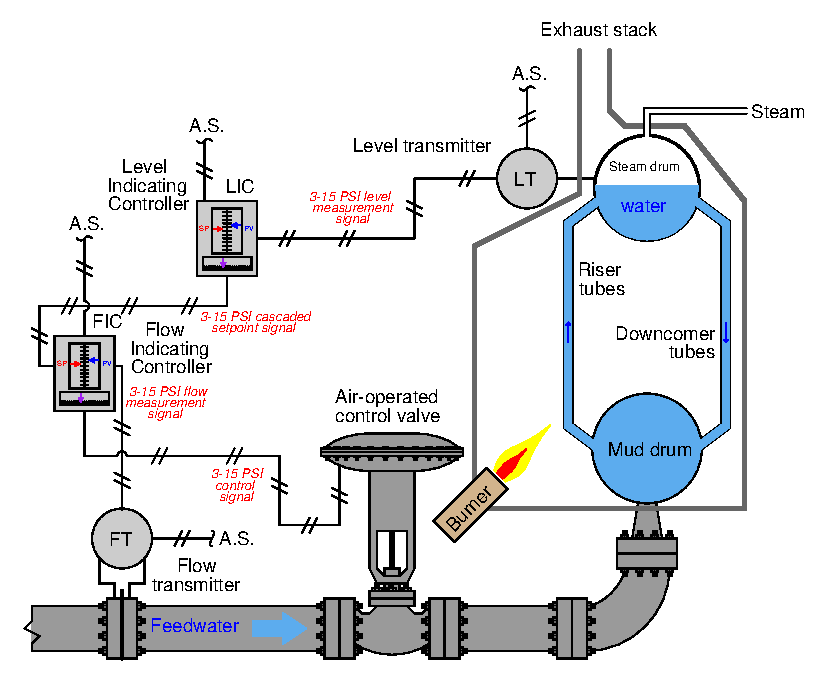
\includegraphics{cont19.eps}$$

The ``secondary'' or ``slave'' flow controller works to maintain feedwater flow to the boiler at whatever flow rate is desired by the level controller.  If feedwater pressure happens to increase or decrease, any resulting changes in flow will be quickly countered by the flow controller without the level controller having to react to a consequent upset in steam drum water level.  Thus, cascade control works to guard against steam drum level instability resulting from changes in the feedwater flow caused by factors outside the boiler.  As stated previously, the slave (flow) controller effectively \textit{shields} the master (level) controller from loads in the feedwater supply system, so that master controller doesn't have to deal with those loads.

This level/flow cascade control system also embodies the principle of the secondary (slave) loop being faster-responding than the primary (master) loop.  Water flow is an inherently fast process, the flow rate responding immediately to changes in valve position.  By contrast, water level is a much slower-responding type of process.  If you perform a ``thought experiment'' where the feedwater valve is suddenly opened fully, it is easy to see that the feedwater flow rate will immediately reach its full (100\%) value while the steam drum's water level will merely begin to rise, taking time to reach its full (100\%) value.

\filbreak

It is worth noting that the inclusion of a flow control ``slave'' loop to this boiler water level control system also helps to overcome a potential problem of the control valve: nonlinear behavior.  In the control valves chapter, we explore the phenomenon of \textit{installed valve characteristics} (Section \ref{installed_valve_characteristic} beginning on page \pageref{installed_valve_characteristic}), specifically noting how changes in pressure drop across a control valve influences its throttling behavior.  The result of these pressure changes is a non-linearization of valve response, such that the valve tends to be more responsive near its closed position and less responsive near its open position.  One of the benefits of cascaded flow control is that this problem becomes confined to the secondary (flow control) loop, and is effectively removed from the primary control loop.  To phrase it simply, distorted valve response becomes ``the flow controller's problem'' rather than something the level controller must manage.  The result is a level control system with more predictable response.  \index{Installed valve characteristic} 

\vskip 10pt

\filbreak

A classic example of cascade control strategy is found in \textit{motion control} applications, where an electric motor is used as the final control element to precisely position a piece of machinery.  In this capacity, the motor is usually called a \textit{servo}.  Robotic systems make extensive use of servo motors and cascaded control loops to modulate power to those motors.  The following illustration shows a triple-cascade control system\footnote{Interestingly, servo motor control is one application where \textit{analog} loop controllers have historically been favored over digital loop controllers, simply for their superior speed.  An opamp-based P, PI, or PID controller is lightning-fast because it has no need to digitize any analog process variables (analog-to-digital conversion) nor does it require time for a clock to sequence step-by-step through a written program as a microprocessor does.  Servomechanism processes are inherently fast-responding, and so the controller(s) used to control servos must be faster yet.} for a motor-actuated elevator, precisely controlling the position of the elevator through cascaded velocity and motor current control:  \index{Motion control system}  \index{Triple-cascaded loops}  \index{Servo motor control}

$$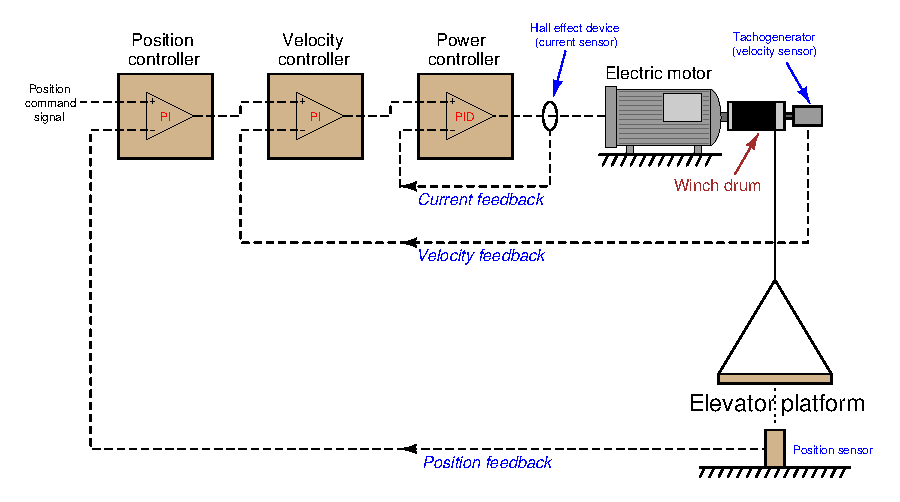
\includegraphics{cont75.eps}$$

Hypothetically, the position of the elevator could be controlled with a single PID controller sensing platform position and directly sending power to the motor.  However, much more precise control of the platform is achievable by sensing position, velocity, and motor current, and controlling each one of those variables with its own loop.  In motion control systems, each successive variable is the time-derivative of its precursor.  Velocity, for instance, is the time-derivative of position ($v = {dx \over dt}$).  Motor current, which is usually proportional to motor torque, which in turn is proportional to the angular acceleration ($\alpha$) of the winch and consequently the linear acceleration of the platform ($a$), is the time-derivative of velocity ($a = {dv \over dt}$).  If it were not for cascading, a single PID controller would have to control position by manipulating the \textit{acceleration} of the platform (i.e. motor current).  This would make the process characteristic ``runaway'' in nature, as any fixed amount of current will cause the platform to accelerate\footnote{At one specific current level, the motor will develop just enough torque to hold the platform's weight, at which point the acceleration will be zero.  Any amount of current above this value will cause an upward acceleration, while any amount of current below this value will cause a downward acceleration.}.

Here with servomechanisms we see how cascading not only has the effect of ``shielding'' certain load variables from the master controller's view, but it also simplifies the dynamic characteristics of the process from that same point of view.  Instead of the position controller having to regulate an inherently ``runaway'' process, it now sees the process as having an ``integrating'' characteristic, since any constant output signal from the position controller results in the platform holding to a constant velocity (i.e. platform position will change at a constant rate over time, rather than at an accelerating rate).

\vskip 10pt

A necessary step in implementing cascade control is to ensure the secondary (``slave'') controller is well-tuned \textit{before} any attempt is made to tune the primary (``master'') controller.  Just a moment's thought is all that is needed to understand why this precedence in tuning must be: it is a simple matter of dependence.  The slave controller does not depend on good tuning in the master controller in order to control the slave loop.  If the master controller were placed in manual (effectively turning off its automatic response), the slave controller would simply control to a constant setpoint.  However, the master controller most definitely depends on the slave controller being well-tuned in order to fulfill the master's ``expectations.''  If the slave controller were placed in manual mode, the master controller would not be able to exert any control over its process variable whatsoever.  Clearly then, the slave controller's response is essential to the master controller being able to control its process variable, therefore the slave controller should be tuned first when initially commissioning or optimizing a cascade control system.

\vskip 10pt

Just like supervisory control systems where a process controller receives a ``remote'' setpoint signal from some other system, the secondary (``slave'') controller in a cascade system typically has three different operating modes:

\begin{itemize}
\item \textbf{Manual mode:} Controller takes no automatic action.  Output value set by human operator.
\item \textbf{Automatic mode:} Controller automatically adjusts its output to try to keep PV = SP.  Setpoint value set ``locally'' by human operator.
\item \textbf{Cascade mode:} Controller automatically adjusts its output to try to keep PV = SP.  Setpoint value set ``remotely'' by primary (master) controller.
\end{itemize}

This means it is possible to defeat a cascade control system by placing the secondary controller in the wrong mode (automatic) just as it is possible to defeat any control system by placing the controller in manual mode.  If a controller is ``slaved'' to another controller, it must be left in \textit{cascade} mode in order for the control strategy to function as designed.

% ADD: discuss how cascaded flow systems may result in shifting the characteristics of a process from self-regulating (with lag) to purely integrating.











\filbreak
\section{Ratio control}

Most people reading this book have likely had the experience of adjusting water temperature using two hand valves as they took a shower: one valve controlling the flow of hot water and the other valve controlling the flow of cold water.  In order to adjust water temperature, the \textit{proportion} of one valve opening to the other must be changed.  Increasing or decreasing total water flow rate without upsetting the outlet temperature is a matter of adjusting both valves in the same direction, maintaining that same proportion of hot to cold water flow.

Although you may not have given it much thought while taking your shower, you were engaged in a control strategy known as \textit{ratio control}, where the ratio of one flow rate to another is controlled for some desired outcome.  Many industrial processes also require the precise mixing of two or more ingredients to produce a desired product.  Not only do these ingredients need to be mixed in proper proportion, but it is usually desirable to have precise control over the total flow rate as well.  \index{Ratio control strategy}

A simple example of ratio control is in the production of paint, where a base liquid must be mixed with one or more pigments to achieve a desired consistency and color.  A manually controlled paint mixing process, similar to the hot and cold water valve ``process'' in some home showers, is shown here.  Two flowmeters, a ratio calculating relay, and a display provide the human operator with a live measurement of pigment-to-base ratio:

$$\includegraphics{cont22.eps}$$

\filbreak

One alteration we could make to this mixing system is to link the two manual control valve handles together in such a way that the ratio of base to pigment was \textit{mechanically} established.  All the human operator needs to do now is move the one link to increase or decrease mixed paint production:

$$\includegraphics{cont23.eps}$$

Adjusting the pigment-to-base ratio is now a matter of adjusting the linkage ratio, a task most likely performed by a mechanic or someone else skilled in the alignment of mechanical linkages.  The convenience of total flow adjustment gained by the link comes at the price of inconvenient ratio adjustment.

\filbreak

Mechanical link ratio-control systems are commonly used to manage simple burners, proportioning the flow rates of fuel and air for clean, efficient combustion.  A photograph of such a system appears here, showing how the fuel gas valve and air damper motions are coordinated by a single rotary actuator:

$$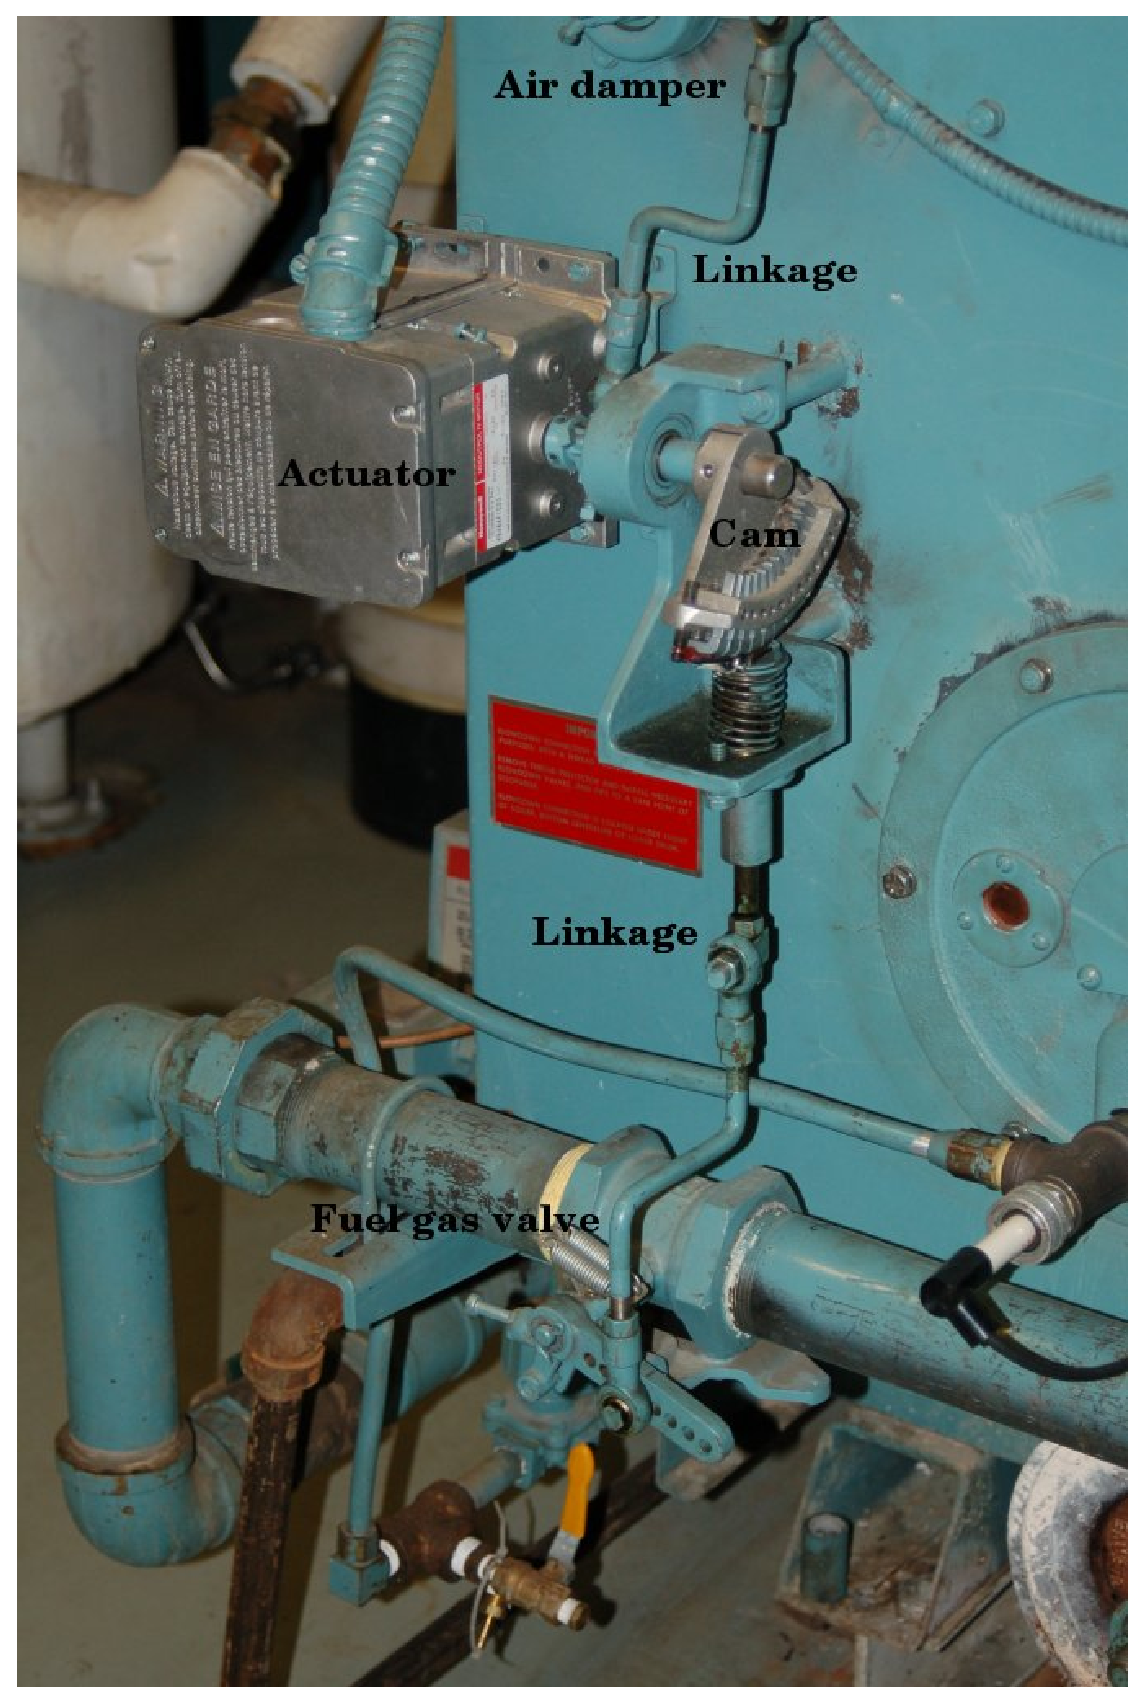
\includegraphics[width=4in]{cont67.eps}$$

As you can see in this photo, the fuel gas valve is actuated by means of a cam, allowing precise ``tuning'' of the valve characteristics for consistent fuel/air ratio across a wide range of firing rates.  Making ratio adjustments in such a linkage system is obviously a task for a skilled mechanic or technician.

\filbreak

A more automated approach to the general problem of ratio control involves the installation of a flow control loop on one of the lines and a flow-sensing transmitter on the other line.  The signal coming from the uncontrolled flow transmitter becomes the setpoint for the flow control loop:

$$\includegraphics{cont24.eps}$$

Here, the flow transmitter on the uncontrolled line measures the flow rate of base, sending a flow rate signal to the pigment flow controller which acts to match flow rates.  If the calibrations of each flow transmitter are precisely equal to one another, the ratio of pigment to base will be 1:1 (equal).  The flow of base liquid into the mixing system is called a \textit{wild flow} or \textit{wild variable}, since this flow rate is not controlled by the ratio control system.  The only purpose served by the ratio control system is to match the pigment flow rate to the wild (base) flow rate, so the same ratio of pigment to base will always be maintained regardless of total flow rate.  Thus, the flow rate of pigment will be held \textit{captive} to match the ``wild'' base flow rate, which is why the controlled variable in a ratio system is sometimes called the \textit{captive variable} (in this case, a captive \textit{flow}).  \index{Wild variable}  \index{Wild flow}  \index{Captive variable}  \index{Captive flow}

As with the mechanically-linked manual ratio mixing system, this ratio control system provides convenient total flow control at the expense of convenient ratio adjustment.  In order to alter the ratio of pigment to base, someone must re-range one or more flow transmitters.  To achieve a 2:1 ratio of base to pigment, for example, the base flow transmitter's range would have to be double that of the pigment flow transmitter.  This way, an equal percentage of flow registered by both flow transmitters (as the ratio controller strives to maintain equal percentage values of flow between pigment and base) would actually result in twice the amount of base flow than pigment flow.

\filbreak

We may incorporate convenient ratio adjustment into this system by adding another component (or function block) to the control scheme: a device called a \textit{signal multiplying relay} (or alternatively, a \textit{ratio station}).  This device (or computer function) takes the flow signal from the base (wild) flow transmitter and multiplies it by some constant value ($k$) before sending the signal to the pigment (captive) flow controller as a setpoint:  \index{Multiplying relay}  \index{Ratio station}

$$\includegraphics{cont25.eps}$$

With identical flow range calibrations in both flow transmitters, this multiplying constant $k$ directly determines the pigment-to-base ratio (i.e. the ratio will be 1:1 when $k=1$; the ratio will be 2:1 when $k=2$, etc.).  If the $k$ value is easily adjusted by a human operator, mixing ratio becomes a very simple parameter to change at will, just as the total production rate is easy to adjust by moving the base flow control valve.

\vskip 10pt

Another example of ratio control at work is in a process whereby hydrocarbon gases (usually methane) are converted into hydrogen gas and carbon dioxide gas.  This is known as the \textit{steam-hydrocarbon reforming process}, and it is one of the more popular ways of generating hydrogen gas for industrial use.  The overall reaction for this process with methane gas (CH$_{4}$) and steam (H$_{2}$O) as the reactants is as follows\footnote{The conversion from hydrocarbon and steam to hydrogen and carbon dioxide is typically a two-stage process: the first (\textit{reforming}) stage produces hydrogen gas and carbon monoxide, while a second (\textit{water-gas-shift}) stage adds more steam to convert the carbon monoxide into carbon dioxide with more hydrogen liberated.  Both reactions are endothermic, with the reforming reaction being more endothermic than the water-gas-shift reaction.}:  \index{Steam-hydrocarbon reforming process}

$$\hbox{CH}_4 + 2\hbox{H}_2\hbox{O} \to 4\hbox{H}_2 + \hbox{CO}_2$$

This is an \textit{endothermic chemical reaction}, which means a net input of energy is required to make it happen.  Typically, the hydrocarbon gas and steam are mixed together in a heated environment in the presence of a catalyst (to reduce the activation energy requirements of the reaction).  This usually takes the form of catalyst-packed metal tubes inside a gas-fired furnace.  It is important to control the proportion of gas to steam flow into this process.  Too much hydrocarbon gas, and the result will be ``coking'' (solid hydrocarbon deposits) inside the heated tubes and on the surface of the catalyst beads, decreasing the efficiency of the process over time.  Too much steam and the result is wasted energy as unreacted steam simply passes through the heater tubes, absorbing heat and carrying it away from the catalyst where it would otherwise do useful work.

One way to achieve the proper ratio of hydrocarbon gas to steam flow is to install a normal flow control loop on one of these two reactant feed lines, then use that process variable (flow) signal as a setpoint to a flow controller installed on the other reactant feed line.  This way, the second controller will maintain a proper balance of flow to proportionately match the flow rate of the other reactant.  An example P\&ID is shown here, where the methane gas flow rate establishes the setpoint for steam flow control:

$$\includegraphics{cont20.eps}$$

Note how the methane gas flow transmitter signal goes both to the methane flow controller and to a \textit{multiplying relay} that multiplies this signal by a constant value ($k$) before passing it on to the steam flow controller as a setpoint.  This $k$ value sets the \textit{ratio} of steam flow to methane flow.  Although this might appear to be a cascade control system at first glance, it is actually quite different.  In a cascade system, the \textit{output} of one controller becomes the setpoint for another.  Here in a ratio control system, the \textit{process variable} of one controller becomes the setpoint for another, such that two process variables remain in constant proportion (ratio) to one another.

If the two flow transmitters are compensated to measure mass flow, the ideal value of $k$ should be set such that two molecules of steam vapor (H$_{2}$O) enter the reforming furnace for every one molecule of methane (CH$_{4}$).  With a 2-to-1 molecular ratio of steam to methane (2 moles of steam per one mole of methane), this equates to a 9-to-4 mass flow ratio once the formula weights of steam and methane are calculated\footnote{Steam has a formula weight of 18 amu per molecule, with two hydrogen atoms (1 amu each) and one oxygen atom (16 amu).  Methane has a formula weight of 16 amu per molecule, with one carbon atom (12 amu) and four hydrogen atoms (1 amu each).  If we wish to have a molecular ratio of 2:1, steam-to-methane, this makes a formula weight ratio of 36:16, or 9:4.}.  Thus, if the methane and gas flowmeters are calibrated for equal mass flow ranges, the ideal value for $k$ should be ${9 \over 4}$, or 2.25.  Alternatively, the flow transmitter calibrations could be set in such a way that the ideal ratio is intrinsic to those transmitters' ranges (i.e. the methane flow transmitter has 2.25 times the mass flow range of the steam flow transmitter), with $k$ set to an ideal value of 1.  This way a 9:4 ratio of methane mass flow to steam mass flow will result in equal percentage output values from both flow transmitters.  In practice, the value for $k$ is set a bit higher than ideal, in order to ensure just a little excess steam to guard against coking inside the reaction heater tubes\footnote{It is quite common for industrial control systems to operate at ratios a little bit ``skewed'' from what is stoichiometrically ideal due to imperfect reaction efficiencies.  Given the fact that no chemical reaction ever goes to 100\% completion, a decision must be made as to which form of incompleteness is worse.  In a steam-hydrocarbon reforming system, we must ask ourselves which is worse: excess (unreacted) steam at the outlet, or excess (unreacted) hydrocarbon at the outlet.  Excess hydrocarbon content will ``coke'' the catalyst and heater tubes, which is very bad for the process over time.  Excess steam merely results in a bit more operating energy loss, with no degradation to equipment life.  The choice, then, is clear: it is better to operate this process ``hydrocarbon-lean'' (more steam than ideal) than ``hydrocarbon-rich'' (less steam than ideal).}.  \index{Formula weight}

\filbreak

We could add another layer of sophistication to this ratio control system by installing a gas analyzer at the outlet of the reaction furnace designed to measure the composition of the product stream.  This analyzer's signal could be used to adjust the value of $k$ so the ratio of steam to methane would automatically vary to ensure optimum production quality even if the feedstock composition (i.e. percentage concentration of methane in the hydrocarbon gas input) changes:

$$\includegraphics{cont21.eps}$$

As we saw before, pure methane feed requires a 9-to-4 steam-to-methane mass flow ratio for the desired reaction to be stoichiometrically balanced.  This mass ratio, however, is not balanced for hydrocarbons other than methane.  Ethane (C$_{2}$H$_{6}$) processed in the same way requires a 12-to-5 steam-to-ethane mass flow ratio.  Propane (C$_{3}$H$_{8}$) requires a 26-to-11 steam-to-propane mass flow ratio.  If the hydrocarbon feed to the reforming furnace varies in composition, the steam flow ratio ($k$) must change accordingly for efficient reaction.








\filbreak
\section{Relation control}

A control strategy similar to ratio control is \textit{relation} control.  This is similar to ratio control in that a ``wild'' variable determines the setpoint for a captive variable, but with relation control the mathematical relationship between the wild and captive variables is one of addition (or subtraction) rather than multiplication (or division).  In other words, a relation control system works to maintain a specific \textit{difference} between wild and captive flow values, whereas a ratio control system works to maintain a specific \textit{ratio} between wild and captive flow values.  \index{Relation control strategy}

An example of relation control appears here, where a temperature controller for a steam superheater on a boiler receives its setpoint from the biased output of a temperature transmitter sensing the temperature of saturated steam (that is, steam exactly at the boiling point of water) in the steam drum:

$$\includegraphics{cont70.eps}$$

It is a basic principle of thermodynamics that the vapor emitted at the surface of a boiling liquid will be at the same temperature as that liquid.  Furthermore, any heat lost from that vapor will cause at least some of that vapor to condense back into liquid.  In order to ensure the vapor is ``dry'' (i.e. it may lose substantial heat energy without condensing), the vapor must be heated beyond the liquid's boiling point at some later stage in the process.

Steam within the steam drum of a boiler is \textit{saturated} steam: at the same temperature as the boiling water.  Any heat lost from saturated steam causes at least some of it to immediately condense back into water.  In order to ensure ``dry'' steam output from the boiler, the saturated steam taken from the steam drum must be further heated through a set of tubes called a \textit{superheater}.  The resulting ``dry'' steam is said to be \textit{superheated}, and the difference between its temperature and the temperature of the boiling water (saturated steam) is called \textit{superheat}.  \index{Superheater}  \index{Superheat}  \index{Superheated steam}

This control system maintains a set amount of superheat by measuring the saturated steam's temperature (within the steam drum), adding a ``superheat setpoint'' bias value to that signal, then passing the biased signal to the temperature indicating controller (TIC) where the superheated steam temperature is regulated by adding water\footnote{This mixing of superheated steam and cold water happens in a specially-designed device called a \textit{desuperheater}.  The basic concept is that the water will absorb heat from the superheated steam, turning that injected water completely into steam and also reducing the temperature of the superheated steam.  The result is a greater volume of steam than before, at a reduced temperature.  So long as some amount of superheat remains, the de-superheated steam will still be ``dry'' (above its condensing temperature).  The desuperheater control merely adds the appropriate amount of water until it achieves the desired superheat value.} to the superheated steam.  With this system in place, the boiler operator may freely define how much superheat is desired, and the controller attempts to maintain the superheated steam at that much higher temperature than the saturated steam in the drum, over a wide range of saturated steam temperatures.  \index{Desuperheater}

A ratio control system would not be appropriate here, since what we desire in this process is a controlled \textit{offset} (rather than a controlled \textit{ratio}) between two steam temperatures.  The control strategy looks very much like a ratio control, except for the substitution of a summing function instead of a multiplying function.








\filbreak
\section{Feedforward control}

``Feedforward'' is a rather under-used control strategy capable of managing a great many types of process problems.  It is based on the principle of \textit{preemptive load counter-action:} that if all significant loads on a process variable are monitored, and their effects on that process variable are well-understood, a control system programmed to take appropriate action based on load changes will shield the process variable from any ill effect.  That is to say, the feedforward control system uses data from load sensors to predict when an upset is about to occur, then \textit{feeds that information forward to the final control element} to counteract the load change before it has an opportunity to affect the process variable.  Feedback control systems are \textit{reactive}, taking action after to changes in the process variable occur.  Feedforward control systems are \textit{proactive}, taking action before changes to the process variable can occur.

This photograph shows a kind of feedforward strategy employed by human operators running a \textit{retort}: a steam-powered machine used to pressure-treat wooden beams at a milled lumber operation.  The sign taped to this control panel reminds the operator to warn the maintenance department of an impending steam usage:

$$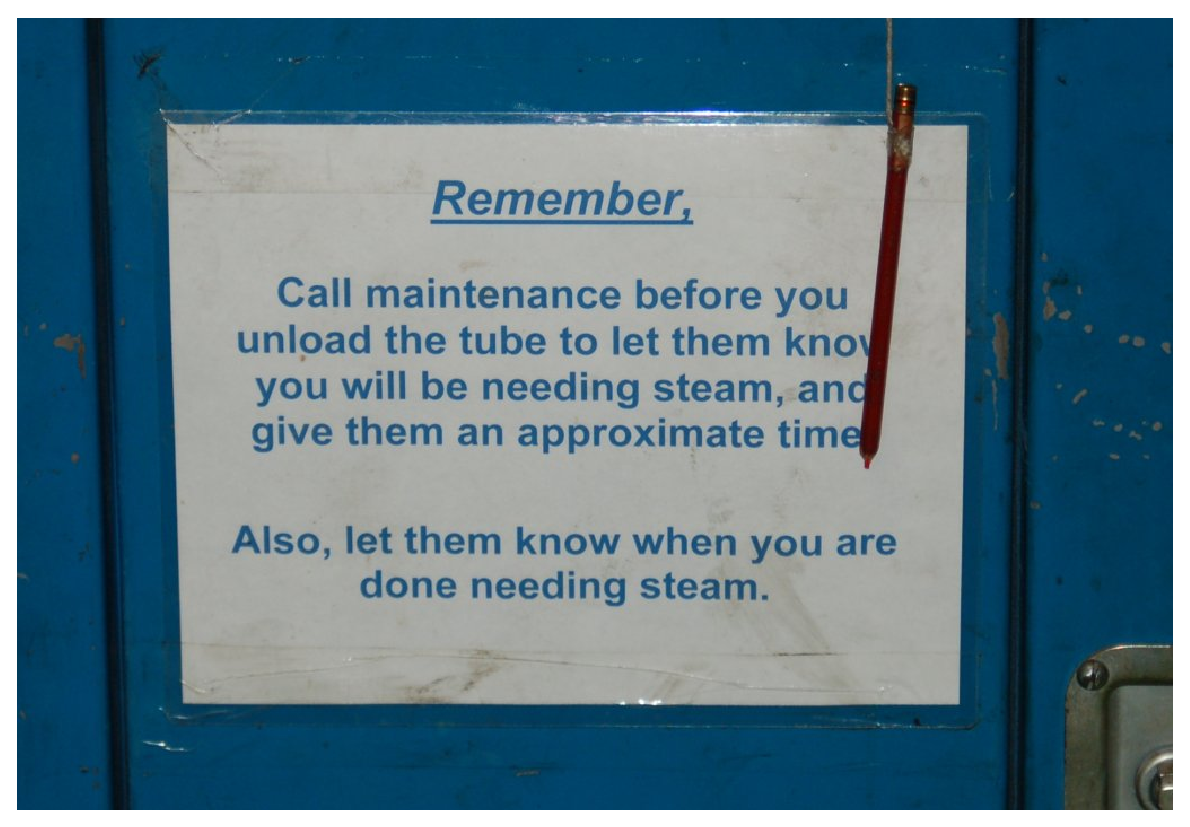
\includegraphics[width=5in]{cont86.eps}$$

The story behind this sign is that a sudden demand in retort steam causes the entire facility's steam supply pressure to sag if it happens at a time when the boiler is idling.  Since the boiler's pressure control system can only react to deviations in steam pressure from setpoint, the boiler pressure controller will not take any action to compensate for sudden demand until \textit{after} it sees the steam pressure fall, at which point it may be too late to fully recover.  If operators give the maintenance personnel advance notice of the steam demand, though, the boiler may be fired up for extra steam capacity and thus will be prepared for the extra demand when it comes.  The upset avoided here is abnormally low steam header pressure, with the predictive load being the retort operator's planned usage of steam.  Crude as this solution might be, it illustrates the fundamental concept of feedforward control: information about a load change is ``fed forward'' to the final control element to preemptively stabilize the process variable.

\vskip 10pt

As the following section explains, perfect feedforward control action is nearly impossible to achieve.  However, even imperfect feedforward action is often far better than none at all, and so this control strategy is quite valuable in process control applications challenged by frequent and/or large variations in load.





\filbreak
\subsection{Load Compensation}

\textit{Feedback} control works on the principle of information from the outlet of a process being ``fed back'' to the input of that process for corrective action.  A block diagram of feedback control looks like a loop:  \index{Feedback control system}

$$\includegraphics{cont05.eps}$$

\filbreak

The reason any control system is necessary at all\footnote{This statement is true only for self-regulating processes.  Integrating and ``runaway'' processes require control systems to achieve stability even in the complete absence of any loads.  However, since self-regulation typifies the vast majority of industrial processes, we may conclude that the fundamental purpose of most control systems is to counteract the effects of loads.} to maintain a process variable at some stable value is the existence of something called a \textit{load}.  A ``load'' is a variable influencing a process that is not itself under direct control, and may be represented in the block diagram as an arrow entering the process, but not within the control loop:  \index{Load, process}  \index{Process load}

$$\includegraphics{cont26.eps}$$

For example, consider the problem of controlling the speed of an automobile.  In this scenario, vehicle speed is the process variable being measured and controlled, while the final control device is the accelerator pedal controlling engine power output.  If it were not for the existence of hills and valleys, head-winds and tail-winds, air temperature changes, road surface variations, and a host of other ``load'' variables affecting car speed, maintaining a constant speed would be as simple as holding the accelerator pedal at a constant position.

However, the presence of these ``load'' variables makes necessitates a human driver (or a \textit{cruise control} system) continually adjusting engine power to maintain constant speed.  Using the car's measured speed as feedback, the driver (or cruise control) adjusts the accelerator pedal position as necessary based on whether or not the car's speed matches the desired ``setpoint'' value.

An inherent weakness of any feedback control system is that it can never be \textit{proactive}.  The best any feedback control system can ever do is \textit{react} to detected disturbances in the process variable.  This makes deviations from setpoint inevitable, even if only for short periods of time.  In the context of our automobile cruise control system, this means the car can never maintain a \textit{perfectly} constant speed in the face of loads because the control system does not have the ability to anticipate loads (e.g. hills, wind gusts, changes in air temperature, changes in road surface, etc.).  At best, all the feedback cruise control system can do is react to changes in speed it senses \textit{after} some load has disturbed it.

\vskip 10pt

\textit{Feedforward} control addresses this weakness by taking a fundamentally different approach, basing final control decisions on the states of load variables rather than the process variable.  In other words, a feedforward control system monitors the factor(s) influencing a process and decides how to compensate \textit{ahead of time} before the process variable deviates from setpoint.  If all loads are accurately measured, and the control algorithm realistic enough to predict process response for these known load values, the process variable (ideally) need not be measured at all:  \index{Feedforward control strategy}

$$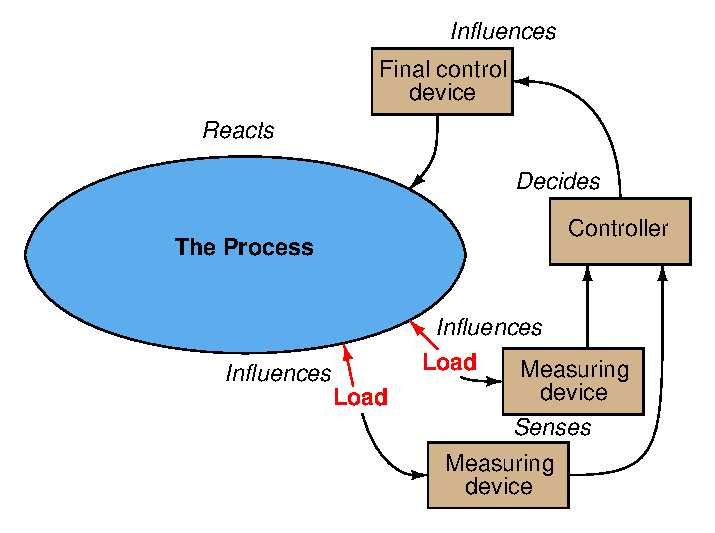
\includegraphics{cont27.eps}$$

As was the case with cascade control, feedforward control also has an analogue in workplace management.  If you consider a supervisor to be the ``controller'' of a work group (issuing orders to his or her subordinates to accomplish important tasks), a feedforward system would be when someone informs the supervisor of an important change that will soon impact the work group.  By having this information ``fed forward'' to the supervisor, the supervisor may then take \textit{preemptive} measures to better manage this change before its effects are fully felt.  If this predictive information is accurate, and the supervisor's response appropriate, any negative impacts of the change will be minimized to the point where no reactive steps will be needed.  Stated differently, good feedforward control action translates what would otherwise be a crisis into an insignificant event.

Returning to the cruise control application, a purely feedforward automobile cruise control system would be interfaced with topographical maps, real-time weather monitors, and road surface sensors to decide how much engine power was necessary at any given time to attain the desired speed\footnote{The load variables I keep mentioning that influence a car's speed constitute an incomplete list at best.  Many other variables come into play, such as fuel quality, engine tuning, and tire pressure, just to name a few.  In order for a purely feedforward (i.e. no feedback monitoring of the process variable) control system to work, \textit{every single load variable} must be accurately monitored and factored into the system's output signal.  This is impractical or impossible for a great many applications, which is why we usually find feedforward control used in conjunction with feedback control, rather than feedforward control used alone.}.  Assuming all relevant load variables are accounted for, the cruise control would be able to maintain constant speed regardless of conditions, and without the need to even monitor the car's speed.

This is the promise of feedforward control: a method of controlling a process variable so perfect in its predictive power that it eliminates the need to even measure that process variable.  If you are skeptical of this feedforward principle and its ability to control a process variable without even measuring it, this is a good thing -- you are thinking critically!  In practice, it is nearly impossible to accurately account for \textit{all} loads influencing a process and to both anticipate and counter-act their combined effects, and so \textit{pure} feedforward control systems are rare\footnote{In fact, the only pure feedforward control strategies I have ever seen have been in cases where the process variable was nearly impossible to measure and could only be inferred from other variables.}.  Instead, the feedforward principle finds use as a supplement to normal feedback control.  To understand feedforward control better, however, we will consider its pure application before exploring how it may be combined with feedback control.

\vskip 10pt

\filbreak

First, let us consider a liquid level control system on an open tank, where three different fluid ingredients (shown in the following P\&ID simply as A, B, and C) are mixed to produce a final product.  A level transmitter (LT) measures liquid level, while a level controller (LC) compares this level to a setpoint value, and outputs a signal calling for a certain amount of discharge flow.  A cascaded (slave) flow controller (FC) senses outgoing flow via a flow transmitter (FT) and works to maintain whatever rate of flow is ``asked'' for by the level controller:

$$\includegraphics{cont28.eps}$$

The level control system acts to keep liquid level constant in the vessel, ensuring adequate mixing of the three ingredients\footnote{If the liquid level drops too low, there will be insufficient \textit{retention time} in the vessel for the fluids to mix before they exit the product line at the bottom.}.  Being a feedback level control system, it adjusts the discharge flow rate in response to measured changes in liquid level.  Like all feedback control systems, this one is \textit{reactive} in nature: it can only take corrective action \textit{after} a deviation between process variable (level) and setpoint is detected.  As a result, temporary deviations from setpoint are guaranteed to occur with this control system every time the combined flow rate of the three ingredients increases or decreases.  \index{Retention time}

Let us now change the control system strategy from feedback to feedforward.  It is clear what the loads are in this process: the three ingredient flows entering the vessel.  If we measure and sum these three flow rates\footnote{The device or computer function performing the summation is shown in the P\&ID as a bubble with ``FY'' as the label.  The letter ``F'' denotes \textit{Flow}, while the letter ``Y'' denotes a signal relay or transducer.}, then use the total incoming flow signal as a setpoint for the discharge flow controller, the outlet flow should (ideally) match the inlet flow, resulting in a constant liquid level.  Being a purely feedforward control system, there is no level transmitter (LT) any more, just flow transmitters measuring the three loads:

$$\includegraphics{cont29.eps}$$

If all flow transmitter calibrations are perfect, the summing of flow rates flawless, and the flow controller's tuning robust, this level control system should control liquid level in the vessel by proactive effort (``thinking ahead'') rather than reactive effort (``after the fact'').  Any change in the flow rate of ingredients A, B, and/or C is quickly matched by an equal adjustment to the discharge flow rate.  So long as total volumetric flow out of the vessel is held equal to total volumetric flow into the vessel, the liquid level inside the vessel \textit{cannot} change\footnote{Incidentally, this is a good example of an \textit{integrating} mass-balance process, where the rate of process variable change over time is proportional to the imbalance of flow rates in and out of the process.  Stated another way, total accumulated (or lost) mass in a mass-balance system such as this is the time-integral of the difference between incoming and outgoing mass flow rates: $\Delta m = \int_0^T (W_{in} - W_{out}) \> dt$.}.

If this feedforward strategy reminds you of ratio control, you are thinking correctly: the ingredient flow sum signal is the \textit{wild variable}, and the discharge flow signal is the \textit{captive variable}.  The flow controller simply maintains the discharge flow rate at a 1:1 ratio with the (total) ingredient flow rate.  In fact, pure feedforward control is a variation of 1:1 ratio control, except that the real process variable (tank level) is neither the wild (total incoming flow) nor the captive variable (discharge flow) in the process.

\vskip 10pt

An interesting property of feedforward and ratio control systems alike is that they cannot generate oscillations as is the case with an over-tuned (excessive gain) feedback system.  Since a feedforward system does not monitor the effects of its actions, it cannot react to something it did to the process, which is the root cause of feedback oscillation.  While it is entirely possible for a feedforward control system to be configured with too much gain, the effect of this will be \textit{overcompensation} for a load change rather than oscillation.  In the case of the mixing tank feedforward level control process, improper instrument scaling and/or offsets will merely cause the discharge and inlet flows to mis-match, resulting in a liquid level that either continues to increase or decrease over time (``integrate'').  However, no amount of mis-adjustment can cause this feedforward system to produce \textit{oscillations} in the liquid level.

In reality, this pure feedforward control system is impractical even if all instrument calibrations and control calculations are perfect.  There are still loads unaccounted for: evaporation of liquid from the vessel, for example, or the occasional pipe fitting leak.  Furthermore, since the control system has no ``knowledge'' of the actual liquid level, it cannot make adjustments to that level.  If an operator, for instance, desired to decrease the liquid level in order to reduce the residence time (also known as ``retention time'')\footnote{\textit{Residence time} or \textit{Retention time} is the average amount of time each liquid molecule spends inside the vessel.  It is an important variable in chemical reaction processes, where adequate time must be given to the reactant molecules in order to ensure a complete reaction.  It is also important for non-reactive mixing processes such as paint and food manufacturing, to ensure the ingredients are thoroughly mixed together and not stratified.  For any given flow rate through a vessel, the residence time is directly proportional to the volume of liquid contained in that vessel: double the captive volume, and you double the residence time.  For any given captive volume, the residence time is inversely proportional to the flow rate through the vessel: double the flow rate through the vessel, and you halve the residence time.  In some mixing systems where residence time is critical to the thorough mixing of liquids, vessel level control may be coupled to measured flow rate, such that an increase in flow rate results in an increased level setpoint, thus maintaining a constant residence time despite changes in production rate.}, he or she would have to manually drain liquid out of the vessel, or temporarily place the discharge flow controller in ``manual'' mode and increase the flow there (then place back into ``cascade'' mode where it follows the remote setpoint signal again).  The advantage of proactive control and minimum deviation from setpoint over time comes at a fairly high price of impracticality and inconvenience.  \index{Retention time}  \index{Residence time, see Retention time}

\filbreak

For these reasons, feedforward control is most often found in conjunction with feedback control.  To show how this would work in the liquid level control system, we will incorporate a level transmitter and level controller back into the system, the output of that level controller being summed with the feedforward flow signal (by the LY summing relay) before going to the cascaded setpoint input of the discharge flow controller:

$$\includegraphics{cont30.eps}$$

This hybrid control strategy is sometimes called \textit{feedforward with trim}.  In this context, ``trim'' refers to the level controller's (LC) output signal contributing to the discharge flow setpoint, helping to compensate for any unaccounted loads (evaporation, leaks) and provide for level setpoint changes.  This ``trim'' signal should do very little of the control work in this system, the bulk of the liquid level stability coming from the feedforward signals provided by the incoming flow transmitters.  \index{Feedforward with trim}  \index{Trim, in a feedforward control system}

%\filbreak

% ADD: elaborate on feedforward with trim versus ratio with trim.

%Recall how pure feedforward control in its simplest form (having no feedback) was likened to a ratio control system with a fixed 1:1 ratio.  With the addition of feedback (trim) to feedforward, we see something that is truly different from what ratio control looked like with the addition of feedback.  In a ratio control system having feedback, the feedback altered the ratio between wild and captive variables.  In a feedforward control system, the feedback merely \textit{offsets} the wild and captive variables.  Using functional diagrams to illustrate:

%$$\includegraphics{.eps}$$

\filbreak

A very similar control strategy commonly used on large steam boilers for the precise control of steam drum water level goes by the name of \textit{three-element feedwater control}.  The following illustration shows an example of this control strategy implemented with pneumatic (3-15 PSI signal) instruments:  \index{Three-element boiler feedwater control}  \index{3-element boiler feedwater control}  \index{Three-element boiler feedwater control}

$$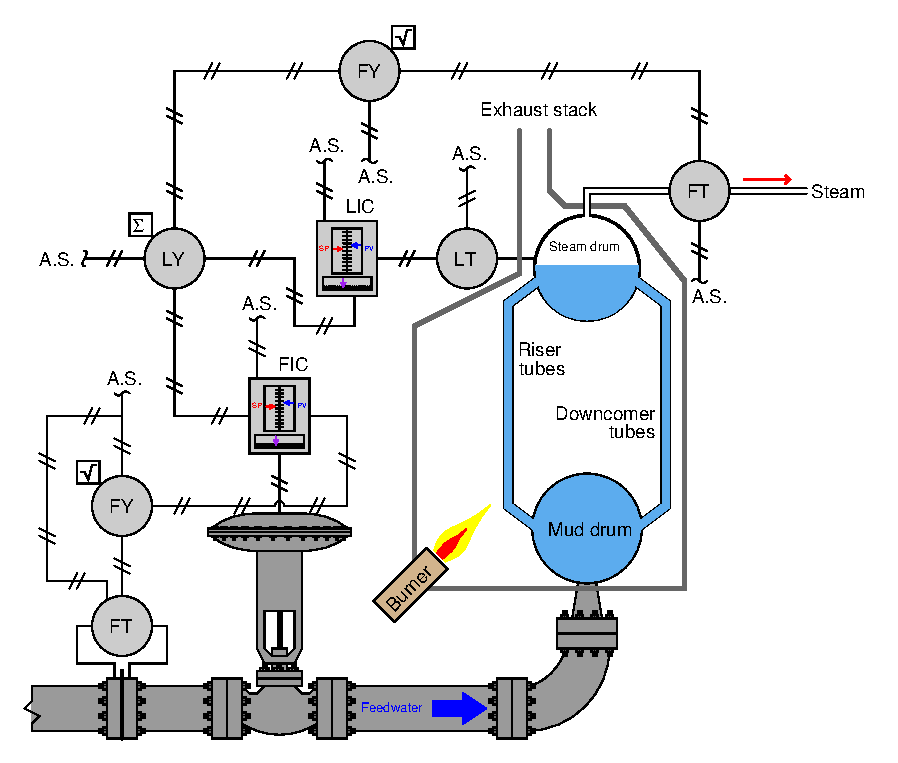
\includegraphics{cont31.eps}$$

Such a control system is called ``three-element'' because it makes use of three process measurements:

\begin{itemize}
\item Feedwater flow rate
\item Steam drum water level
\item Steam flow rate
\end{itemize}

Feedwater flow is controlled by a dedicated flow controller (FIC), receiving a remote setpoint signal from a summing relay (LY).  The summer receives two inputs: a steam flow signal and the output signal (trim) from the level controller (LIC).  The feedforward portion of this system (steam flow feeding forward to water flow) is intended to match the mass flow rates of water into the boiler with steam flow out of the boiler.  If steam demand suddenly increases, this feedforward portion of the system immediately calls for a matching increase in water flow into the boiler, since every molecule of steam exiting the boiler must come from one molecule of water entering the boiler.  The level controller and transmitter act as a feedback control loop, supplementing the feedforward signal to the cascaded water flow controller to make up for (``trim'') any shortcomings of the feedforward loop.

\vskip 10pt

A three-element boiler feedwater control system is a good example of a feedforward strategy designed to ensure \textit{mass balance}, defined as a state of equality between all incoming mass flow rates and all outgoing mass flow rates.  The steam flow transmitter measures outgoing mass flow, its signal being used to adjust incoming water mass rate.  Since mass cannot be created or destroyed (the Law of Mass Conservation), every unit of steam mass leaving the boiler must be accounted for as an equivalent unit of water mass entering the boiler.  If the control system perfectly balances these mass flow rates, water level inside the boiler \textit{cannot} change.  \index{Mass balance}  \index{Conservation of Mass} 

In processes where the process variable is affected by energy flow rates rather than mass, the balance maintained by a feedforward control system will be \textit{energy balance} rather than mass balance.  Like mass, energy cannot be created or destroyed (the Law of Energy Conservation), but must be accounted for.  A feedforward control system monitoring all incoming energy flows into a process and adjusting the outgoing energy flow rate (or vice-versa) will ensure no energy is depleted from or accumulated within the process, thus ensuring the stability of the processes' internal energy state.   \index{Energy balance}  \index{Conservation of Energy}

\filbreak

An example of energy-balance feedforward control appears in this heat exchanger temperature control system:

$$\includegraphics{cont69.eps}$$

The two transmitters on the incoming (cold oil) line measure oil temperature and oil flow rate, respectively.  The first ``summing'' function subtracts the incoming oil temperature from the setpoint (desired) temperature, and then the difference of these two temperatures is then multiplied by the flow rate signal to produce a signal representing the \textit{energy demand}\footnote{Energy demand is an example of what is called an \textit{inferred variable}: a physical quantity that we cannot measure directly but instead calculate from measurements made of other variables.} of the incoming oil (i.e. how much energy will be required to elevate the oil flow's temperature to setpoint).  The ``energy demand'' signal is summed with the temperature controller's output signal to set the steam valve position (adding energy to the process).  \index{Inferred variable}

There do exist other loads in this process, such as ambient air temperature and chemical composition of the oil, but these variables are generally less influential on discharge temperature than feed temperature and flow rate.  This illustrates a practical facet of feedforward control: although there may be a great many loads affecting our process variable, we must generally limit our application of feedforward to only the most dominant loads in order to limit control system cost.  Simply put, we usually cannot justify the expense and complexity of a feedforward control system compensating for \textit{every single load} in a system.




\filbreak
\subsection{Proportioning feedforward action}

Feedforward control works by directly modulating the manipulated variable in a control system according to changes sensed in the load(s).  In order for feedforward to function optimally, it must adjust the manipulated variable in a manner that is proportionate to the need: no more, and no less.  At this juncture it is appropriate to ask the question, ``how do we know the amount of feedforward action that will be adequate for a process, and how do we adjust it if it is too much or too little?''

In processes where the feedforward control strategy attempts to achieve direct mass- or energy-balance, the question of adequate feedforward action is answered in the mathematics of measuring the incoming and outgoing flows.  Consider the following mass-balance level control system where the combined sum of three inlet flows is routed to the setpoint of the exit flow control loop.  In this diagram, the portions of the control strategy implemented as function blocks (algorithms in software) appear inside a yellow-colored bounded area, while all real physical instruments appear outside the yellow area:

$$\includegraphics{cont79.eps}$$

If all flowmeters are calibrated in pounds per minute, then the feedforward signal will likewise be scaled in pounds per minute, and so will the setpoint be for flow control loop.  In a digital control system, it is quite customary to scale each and every analog input signal with some real ``engineering unit'' of measurement, so that the signal will be treated as a physical quantity throughout as opposed to being treated as some anonymous percentage value.  Not only is this consistent scaling a standard feature in digital control systems, but it also helps the implementation of this feedforward control strategy, because we desire the out-going mass flow rate to precisely match the (total) in-coming flow rate.  So long as all flowmeters and their associated scaling factors are accurate, the feedforward control's action \textit{must} be exactly right: an increase of +5 pounds per minute in incoming flow rate will prompt an immediate increase of +5 pounds per minute in outgoing flow rate, simply by virtue of all these measured flows having been scaled in the same unit of measurement.

\vskip 10pt

\filbreak

The situation is not as simple in systems where the feedforward control is not precisely balancing mass-flow or energy rates.  By contrast, let us examine the following pH neutralization system equipped with feedforward control action.  Here, the incoming liquid is alkaline (pH greater than 7), and the control system's job is to mix just enough acid reagent to ``neutralize'' the solution (bring the pH value down to 7):

$$\includegraphics{cont80.eps}$$

Controlling the pH (acidity/alkalinity) of a liquid solution is challenging for many reasons, not the least of which being the need to have adequate mixing time for the reagent to react with the influent.  This mixing time translates to \textit{dead time} in the feedback control system.  If the influent's pH suddenly changes for any reason, the feedback control system will be slow to alter the reagent flow rate due to this dead time, causing long-lasting deviations from setpoint.  The goal of the feedforward signal (from the influent pH transmitter to the summer) is to preemptively adjust reagent flow rate according to how alkaline the incoming flow is, countering any sudden changes in influent pH so the feedback control system doesn't have to take (delayed) action.

Once again, it is appropriate to ask the question, ``how do we know the amount of feedforward action that will be adequate for this process, and how do we adjust it if it is too much or too little?''  It would be blind luck if the system happened to work perfectly as shown, with the influent pH transmitter's signal going straight to the summing function to be added to the pH controller's output signal.  Certainly, an increase in influent pH would cause more acid to be added to the mix thanks to feedforward action, but it would likely add either too much or too little acid than it should.  The scale of the influent pH transmitter does not match the scale of the signal sent to the control valve, and so we do not have a neat ``pound-for-pound'' balance of mass flow as we did in the case of the level control system.  

A neat solution to this problem is to add another function block to the feedforward portion of the control system.  This block takes the influent pH transmitter signal and skews it using multiplication and addition, using the familiar linear equation $y = mx + b$ (where $y$ is the output signal of the function and $x$ is the input signal; $m$ and $b$ being constants).  This function block is typically called a \textit{gain and bias} block:  \index{Gain and bias function block}

$$\includegraphics{cont81.eps}$$

The gain adjustment ($m$) in this function block serves to amplify or attenuate the feedforward signal's magnitude, while the bias adjustment ($b$) offsets it.  

\filbreak

Determining practical values for these ``feedforward tuning constants'' is relatively easy.  First, disable feedback control\footnote{Most control systems' feedforward function blocks are designed in such a way that both the feedback and the feedforward signal paths are disabled when the controller is placed into manual mode, in order to give the human operator 100\% control over the final element (valve) in that mode.  For the purpose of ``tuning'' the feedforward gain/bias function block, one must disable the feedback control \textit{only} so feedforward action is still able to respond to load changes.  If simply switching the feedback controller to manual mode is not an option (which it usually is not), one may achieve the equivalent result by setting the gain value of the feedback controller to zero and ensuring the PID equation is not the ``parallel'' type.  If the PID equation is parallel, you will need to set all three terms (P, I, and D) at their minimum settings.} with the output value at or near 50\%.  Next, introduce load changes to the process while watching the process variable's value after sufficient time has elapsed to see the effects of those load changes.  Increase or decrease the gain value until step-changes in load cease to yield significant changes in the process variable.  The following trends show what too much and too little feedforward gain would look like in this pH control system:

$$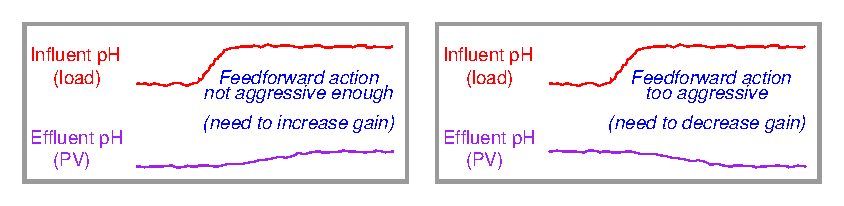
\includegraphics{cont82.eps}$$

If the gain is properly set in the gain/bias function block, these load changes should have minimal effect on the process variable.  Step-changes in influent pH should have little effect on the process variable after sufficient time has passed for the load change to have fully propagated through the process.

Once a good gain value has been found, change the bias value until the process variable approaches the normal setpoint value\footnote{This is why it was recommended to leave the feedback controller's output at or near 50\%.  The goal is to have the feedforward action adjusted such that the feedback controller's output is ``neutral,'' and has room to swing either direction if needed to provide necessary trim to the process.}.  

\vskip 10pt

\filbreak

Some control systems provide convenient methods of incorporating feedforward action.  The standard FOUNDATION Fieldbus PID function block, for example, has its own dedicated signal input for feedforward, with feedforward gain as an existing parameter.  The following illustration shows Fieldbus function blocks used to implement normal feedback (PID) control, and also PID with feedforward control: \index{FOUNDATION Fieldbus}

$$\includegraphics{cont99.eps}$$

As you can see, all that is required to augment a FOUNDATION Fieldbus control system with feedforward control action is the addition of one more analog input (AI) function block for the load transmitter, and one connecting line between that block and the PID block's ``\texttt{FF\_Val}'' input.

\vskip 10pt

\filbreak

Other control systems require a bit more programming to implement feedforward.  For example, consider the standard ``Factory Configured Option 101'' function block program for basic PID feedback control in a Siemens model 353 panel-mounted loop controller, contrasted against the version necessary for implementing feedforward action:

$$\includegraphics{pid119.eps}$$

Note the necessary addition of \textit{two} ``math'' function blocks as well as the extra analog input block for receiving the feedforward (load variable) transmitter's signal: MTH1 needed to add the load transmitter's feedforward signal to the controller's output signal, and MTH2 needed to ensure output tracking still works properly between the PID and A/M function blocks when the human operator switches between automatic and manual modes.  The amount of feedforward action is specified by the ``gain'' parameter for input B of \textit{both} math function blocks, which means any adjustment to feedforward action must be manually entered in two different places!











\filbreak
\section{Feedforward with dynamic compensation}

As we have seen, feedforward control is a way to improve the stability of a feedback control system in the face of changing loads.  Rather than rely on feedback to make corrective changes to a process only \textit{after} some load change has driven the process variable away from setpoint, feedforward systems monitor the relevant load(s) and use that information to preemptively make stabilizing changes to the final control element such that the process variable will not be affected.  In this way, the feedback loop's role is to merely ``trim'' the process for factors lying outside the realm of the feedforward system.

At least, this is how feedforward control is \textit{supposed} to work.  One way feedforward controls commonly fail to live up to their promise is if the effects of load changes and of manipulated variable changes possess different time lags in their respective effects on the process variable.  This is a problem in feedforward control systems because it means the corrective action called for in response to a change in load will not affect the process variable at the same time, or in the same way over time, as the load will.  In order to correct this problem, we must intelligently insert time lags (or advancing time-based functions called \textit{leads}) into the control system to equalize the time lags of load and feedforward correction.  This is called \textit{dynamic compensation}.  \index{Dynamic compensation}

The following subsections will explore illustrative examples to make both the problem and the solution(s) clear.

\vskip 10pt

A common area of confusion among students first approaching this topic is deciding where to place the dynamic compensation function in a feedforward control system.  The answer to this question is surprisingly simple, although it may seem elusive at first glance.  The key is found in the following principle: \textit{the only time-dynamic we have the ability to alter with our control system is the dynamic of the final control element.}  We cannot alter the time-dynamic of the load's effect on the process variable, as that is strictly a function of process physics.  Therefore, when we test a process employing feedforward control with an eye toward incorporating dynamic compensation, we must measure the time lag of the load's effect on PV and also the time lag of our final control element's effect on PV, then compare those two time lags.  If the final control element's time lag is shorter (quicker) than the load's, then we must add a delay or lag to the feedforward signal so that the final control element's preemptive action does not occur too soon.  If the final control element's time lag is longer (slower) than the load's, then we must either find a way to alter the process itself to decrease the load's time lag, or add a ``lead'' function to the feedforward signal in order to advance the final control element's response and thereby ensure the preemptive action does not occur too late.  \textit{Remember, all we can do with dynamic compensation is alter how the final control element responds (i.e. how slowly or quickly the preemptive action of feedforward occurs).  The load's effect on the process variable is fixed by the physics of the process and therefore lies beyond our direct control.}








\filbreak
\subsection{Dead time compensation}

Examine the following control system P\&ID showing the addition of \textit{flocculant} (a chemical compound used in water treatment to help suspended solids clump together for easier removal by filtering and/or gravity clarification) and \textit{lime} for pH balance.  Flocculant is necessary to expedite the removal of impurities from the water, but some flocculation compounds have the unfortunate effect of decreasing the pH value of the water (turning it more acidic).  If the water's pH value is too low, the flocculant ironically loses its ability to function.  Thus, lime (an alkaline substance -- high pH value) must be added to the water to counter-act the flocculant's effect on pH to ensure efficient flocculation.  Both substances are powders in this water pre-treatment system, metered by variable-speed screw conveyors and carried to the mixing tank by belt-style conveyors:

$$\includegraphics{cont32.eps}$$

The control system shown in this P\&ID consists of a pH analyzer (AT) transmitting a signal to a pH indicating controller (AIC), adjusting the speed of the lime screw conveyor.  The flocculant screw conveyor speed is manually set by a \textit{hand indicating controller} (HIC) -- sometimes known as a \textit{manual loading station} -- adjusted when necessary by experienced water treatment operators who periodically monitor the effectiveness of flocculation in the system.  \index{Manual loading station}  \index{Hand controller}

This simple feedback control system will work fine in steady-state conditions, but if the operator suddenly changes flocculant flow rate into the mixing vessel, there will be a temporary deviation of pH from setpoint before the pH controller is able to find the correct lime flow rate into the vessel to compensate for the change in flocculant flow.  In other words, flocculant feed rate into the mixing tank is a \textit{load} for which the pH control loop must compensate.  

\filbreak

Dynamic response could be greatly improved with the addition of feedforward control to this system:

$$\includegraphics{cont33.eps}$$

Here, the hand controller's signal gets added to the pH controller's output signal to directly influence lime feed rate in addition to acting as a control signal to the flocculant screw conveyor motor drive.  If an operator changes the flocculant feed rate, the lime feed rate will immediately adjust to compensate, \textit{before} any change in pH value takes place in the water.  Ideally, the pH controller need only make minor ``trim'' adjustments to lime feed rate, while the feedforward signal does most of the work in maintaining a steady pH value.  The proper proportioning and offset between flocculant and lime feed rates is established in the gain/bias function, which is ``tuned''\footnote{Tuning this gain/bias block is done with the pH controller in manual mode with its output at 50\%.  The gain value is adjusted such that step-changes in flocculant feed rate have little long-term effect on pH.  The bias value is adjusted until the pH approaches setpoint (even with the pH controller in manual mode).} to ensure the feedforward signal does not over- or under-react, calling for too much (or too little) lime to compensate.

Even if all components in the feedforward system have been calibrated and configured properly, however, a potential problem still lurks in this system which can cause the pH value to temporarily deviate from setpoint following flocculant feed rate changes.  This problem is the \textit{transport delay} -- otherwise known as \textit{dead time} -- inherent to the two belt conveyors transporting both flocculant and lime powder from their respective screw conveyors to the mixing vessel.  If the rotational speed of a screw conveyor changes, the flow rate of powder exiting that screw conveyor will immediately and proportionately change.  However, the belt conveyor imposes a time delay before the new powder feed rate enters the mixing vessel.  In other words, the water in the vessel will not ``see'' the effects of a change in flocculant or lime feed rate until after the \textit{belt conveyor's} time delay has elapsed.  This is not a problem if the dead times of both belt conveyors are exactly equal, since this means any compensatory change in lime feed rate initiated by the feedforward system will reach the water at exactly the same time the new flocculant rate reaches the water.  So long as flocculant and lime feed rates are precisely balanced with one another at the point in time they reach the mixing vessel, pH should remain stable.  But what if their arrival times are not coordinated -- what will happen to pH then?  \index{Dead time}  \index{Transport delay}

Let us engage in a ``thought experiment'' to explore the consequences of the flocculant conveyor belt moving much slower than, and/or being much longer than, the lime conveyor belt.  Suppose the flocculant belt imposed a dead time of 60 seconds on flocculant powder making it to the vessel, while the lime belt only delayed lime powder transit by 5 seconds from screw conveyor to mixing tank.  This would mean changes in flocculant flow (set by the hand controller) would compensate with changes in lime flow \textit{55 seconds too soon}.  Now imagine the human operator making a sudden increase to the flocculant powder feed rate.  The lime feed rate would immediately increase thanks to the efforts of the feedforward system.  However, since the increased flow rate of lime powder will reach the mixing vessel 55 seconds before the increased flow rate of flocculant powder, the effect will be a temporary increase in pH value beginning about 5 seconds after the operator's change, and then a settling of pH value back to setpoint\footnote{This ``thought experiment'' assumes no compensating action on the part of the feedback pH controller for the sake of simplicity.  However, even if we include the pH controller's efforts, the problem does not go away.  As pH rises due to the premature addition of extra lime, the controller will try to reduce the lime feed rate.  This will initially reduce the degree to which pH deviates from setpoint, but then the reverse problem will occur when the increased flocculant enters the vessel 55 seconds later.  Now, the pH will drop below setpoint, and the feedback controller will have to ramp up lime addition (to the amount it was before the additional lime reached the vessel) to achieve setpoint.}, as shown in this timing diagram:  \index{Thought experiment}  \index{Problem-solving technique: thought experiment}

$$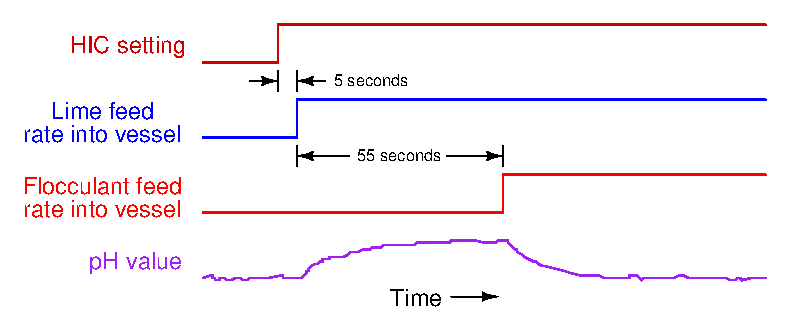
\includegraphics{cont34.eps}$$

The obvious solution to this problem is to mechanically alter the belt conveyor systems for equal transport times of flocculant and lime powders.  If this is impractical, we may achieve a similar result by incorporating another signal relay (or digital function block) inserting dead time into the feedforward control system.  In other words, we can modify the control system in such a way to emulate what would be impractical to modify in the process itself.

\filbreak

This new function will add a dead time of 55 seconds to the feedforward signal before it enters the summer, thus delaying the lime feed rate's response to feedforward effect by just the right amount of time such that any lime feed rate changes called for by feedforward action will arrive at the vessel \textit{simultaneously} with the changed flocculant feed rate:   \index{Dead time function}  \index{Dead time function used for dynamic compensation}

$$\includegraphics{cont35.eps}$$

Adding time-based functions to a control system in order to equalize inherently unequal time delays in the physical process is called \textit{dynamic compensation}.  It is important to note that dynamic compensation cannot make physically unequal time lags equal -- all it does is modify the feedforward system so that signal's effect arrives at the right time to compensate the load.  In simple terms, we can only use dynamic compensation to modify the FCE's behavior, not the process behavior.  Here, there is absolutely nothing the feedforward system can do to speed up the slower flocculant belt, so instead we chose to slow down the feedforward manipulation of lime flow to make it match the flocculant flow.  \index{Dynamic compensation}

Note how the feedback pH controller's loop was purposely spared the effects of the added dead time function, by placing the function outside of that controller's feedback loop.  This is important, as dead time in any form is the bane of feedback control.  The more dead time within a feedback loop, the easier that loop will tend to oscillate.  By strategically placing the dead time function before the summing relay rather than after (between the summer and the lime screw conveyor motor drive), the feedback control system still achieves minimum response time while only the feedforward signal gets delayed.

\vskip 10pt

\filbreak

Let us now consider the same flocculant and lime powder control system, this time with transport delays reversed between the two belt conveyors.  If the flocculant conveyor belt is now the fast one (5 seconds dead time) and the lime belt slow (60 seconds), the effects of flocculant feed rate changes will be reversed.  An increase in flocculant powder feed rate to the vessel will result in a drop in pH beginning 5 seconds after the HIC setting change, followed by a rise in pH value after the additional lime feed rate finally reaches the vessel:

$$\includegraphics{cont36.eps}$$

What is happening here is that the feedforward signal's effect is coming too late.  In a perfect world our lime flow rate into the mixing vessel should change at the same time that the flocculant flow rate changes.  Instead, our lime flow rate's necessary increase happens 55 seconds too late to prevent the pH from deviating.

It would be possible to compensate for the difference in conveyor belt transport times using a special relay in the same location of the feedforward signal path as before, if only there was such a thing as a relay that could \textit{predict the future exactly 55 seconds in advance!}\footnote{Let me know if you are ever able to invent such a thing.  I'll even pay your transportation costs to Stockholm, Sweden so you can collect your Nobel prize.  Of course, I will demand to see the prize before buying tickets for your travel, but with your time-travel device that should not be a problem for you.}.  Since no such device exists (or ever will exist), we must apply dynamic compensation elsewhere in the feedforward control system.

If a time delay is the only type of compensation function at our disposal, then the only thing we can delay in this system to make the two dead times equal is the flocculation feed rate.  Thus, we should place a 55-second dead time relay in the signal path between the hand indicating controller (HIC) and the flocculant screw conveyor motor drive.

\filbreak

This diagram shows the proper placement of the dead time function:  \index{Dead time function used for dynamic compensation}

$$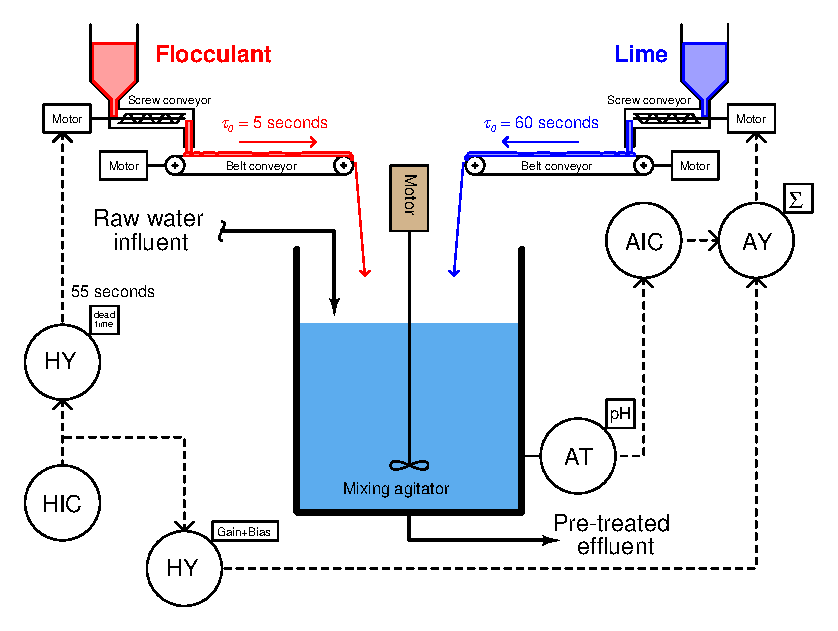
\includegraphics{cont37.eps}$$

With this dead time relay in place, any change in flocculation feed rate initiated by a human operator will immediately adjust the feed rate of lime powder, but delay an adjustment to flocculant powder feed rate by 55 seconds, so the two powders' feed rate changes arrive at the mixing vessel simultaneously.

\vskip 10pt

Bear in mind that this solution will really only work in a system like this where the major load happens to be controlled by the human operator.  In most processes the load variable is not under anyone's control, making it difficult if not impossible to purposely delay its action.  If the load has a shorter dead time than the compensation, there is usually little we can do within the control strategy to equalize those effects for better dynamic stability.  Typically, the best solution is to \textit{physically alter the process} (e.g. slow down the flocculant belt conveyor's speed) so that the load and compensation dead times are closer to being equal.







\filbreak
\subsection{Lag time compensation}

Process time delays characterized by pure transport delay (dead time) are less common in industry than other forms of time delays, most notably \textit{lag times}\footnote{For a more detailed discussion of lag times and their meaning, see section \ref{lag_time} beginning on page \pageref{lag_time}.}.  A simple ``lag'' time is the characteristic exhibited by a low-pass RC filter circuit, where a step-change in input voltage results in an output voltage asymptotically rising to the new voltage value over time:

$$\includegraphics{cont38.eps}$$

The \textit{time constant} ($\tau$) of such a system -- be it an RC circuit or some other physical process -- is the time required for the output to move 63.2\% of the way to its final value ($1 - e^{-1}$).  For an RC circuit such as the one shown, $\tau = RC$ (assuming $R_{load} >> R$ so the load resistance will have negligible effect on timing).  \index{Time constant}  \index{Lag time}

Lag times differ fundamentally from dead times.  With a dead time, the effect is simply time-delayed by a finite amount from the cause, like an echo.  With a lag time, the effect begins at the exact same time as the cause, but does not follow the same rapid change over time as the cause.  Like dead times in a feedforward system, it is quite possible (and in fact usually the case) for loads and final control variables to have differing lag times regarding their respective effects on the process variable.  This presents another form of the same problem we saw in the two-conveyor water pre-treatment system, where an attempt at feedforward control was not completely successful because the corrective feedforward action did not occur with the same amount of time delay as the load.

\filbreak

To illustrate, we will analyze a heat exchanger used to pre-heat fuel oil before being sent to a combustion furnace.  Hot steam is the heating fluid used to pre-heat the oil in the heat exchanger.  As steam gives up its thermal energy to the oil through the walls of the heat exchanger tubes, it undergoes a phase change to liquid form (water), where it exits the shell of the exchanger as ``condensate'' ready to be re-boiled back into steam.  

A simple feedback control system regulates steam flow to the heat exchanger, maintaining the discharge temperature of the oil at a constant setpoint value:

$$\includegraphics{cont39.eps}$$

Once again, it should come as no surprise to us that the outlet temperature will suffer temporary deviations from setpoint if load conditions happen to change.  The feedback control system may be able to \textit{eventually} bring the exiting oil's temperature back to setpoint, but it cannot begin corrective action until \textit{after} a load has driven the oil temperature off setpoint.  What we need for improved control is \textit{feedforward} action in addition to feedback action.  This way, the control system can take corrective action in response to load changes \textit{before} the process variable gets affected.

\filbreak

Suppose we know that the dominant load in this system is oil flow rate\footnote{Knowing this allows us to avoid measuring the incoming cold oil temperature and just measure incoming cold oil flow rate as the feedforward variable.  If the incoming oil's temperature were known to vary substantially over time, we would be forced to measure it as well as flow rate, combining the two variables together to calculate the \textit{energy demand} and use this inferred variable as the feedforward variable.}, caused by changes in demand at the combustion furnace where this oil is being used as fuel.  Adapting this control system to include feedforward is as simple as installing an oil flow transmitter, a gain/bias function, and a summing function block:  \index{Inferred variable}  \index{Gain and bias function block}

$$\includegraphics{cont40.eps}$$

With feedforward control action in place, the steam flow rate will immediately change with oil flow rate, preemptively compensating for the increased or decreased heat demand of the oil.  In other words, the feedforward system attempts to maintain \textit{energy balance} in the process, with the goal of stabilizing the outlet temperature:

There is a problem of time delay in this system, however: a change in oil flow rate has a \textit{faster} effect on outlet temperature than a proportional change in steam flow rate.  This is due to the relative masses impacting the temperature of each fluid.  The oil's temperature is primarily coupled to the temperature of the tubes, whereas the steam's temperature is coupled to both the tubes and the shell of the heat exchanger.  So, the steam has a greater mass to heat than the oil has to cool, giving the steam a larger thermal time constant than the oil.  

For the sake of illustration, we will assume transport delays are short enough to ignore\footnote{Transport delay (dead time) in heat exchanger systems can be a thorny problem to overcome, as they they tend to change with flow rate!  For reasons of simplicity in our illustration, we will treat this process as if it only possessed lag times, not dead times.}, so we are only dealing with different \textit{lag} times between the oil flow's effect on temperature and the steam flow's effect on temperature.

\vskip 10pt

This is what would happen to the heated oil temperature if steam flow were held constant and oil flow were suddenly increased:

$$\includegraphics{cont41.eps}$$

Increased oil flow convects heat away from the steam at a faster rate than before, resulting in decreased oil temperature.  This drop in temperature is fairly quick, and is self-regulating.

\vskip 10pt

By contrast, this is what would happen to the heated oil temperature if oil flow were held constant and steam flow were suddenly increased:

$$\includegraphics{cont42.eps}$$

Increased steam flow convects heat into the oil at a faster rate than before, resulting in increased oil temperature.  This rise in temperature is also self-regulating, but much slower than the temperature change resulting from a proportional adjustment in oil flow.  In other words, the time constant ($\tau$) of the process with regard to steam flow changes is greater than the time constant of the process with regard to oil flow changes ($\tau_{steam} > \tau_{oil}$).

\filbreak

If we superimpose these two effects, as will be the case when the feedforward system is working (without the benefit of feedback ``trim'' control), what we will see when oil flow suddenly increases is a ``fight'' between the cooling effect of the increased oil flow and the heating effect of the increased steam flow.  However, it will not be a fair fight: the oil flow's effect will temporarily win over the steam's effect because of the oil's faster time constant.  Another way of stating this is to say the feedforward action \textit{temporarily under-compensates} for the change in load.  The result will be a momentary dip in outlet temperature before the system achieves equilibrium again:

$$\includegraphics{cont43.eps}$$

The solution to this problem is not unlike the solution we applied to the water treatment system: we must somehow equalize these two lag times so their superimposed effects will directly cancel, resulting in an undisturbed process variable.  An approximate solution for equalizing two different lag times is to cascade two lags together in order to emulate one larger lag time\footnote{Technically, two cascaded lag times is not the same as one large lag time, no matter the time constant values.  Two first-order lags in series with one another create a \textit{second-order lag}, which is a different effect.  However imperfect as the added lag solution is, it is still better than nothing at all!}.  This may be done by inserting a lag time relay or function block in the feedforward system.  \index{Lag time function}

When we look at our P\&ID, though, a problem is immediately evident.  The lag time we need to slow down is the lag time of the oil flow's effect on temperature.  In this system, oil flow is a wild variable, not something we have the ability to control (or delay at will).  Our feedforward control system can only manipulate the steam valve position in response to oil flow, not influence oil flow in order to give the steam time to ``catch up.''

If we cannot slow down the time constant inherent to the wild variable (oil flow), then the best we can do is speed up the time constant of the variable we do have influence over (steam flow).  The solution is to insert something called a \textit{lead function} into the feedforward signal driving the steam valve.  A ``lead'' is the mathematical inverse of a lag.  If a lag is modeled by an RC low-pass filter circuit, then a ``lead'' is modeled by an RC high-pass filter circuit:   \index{Lead time function}  \index{Lead function used for dynamic compensation}

$$\includegraphics{cont44.eps}$$

Being mathematical inverses of each other, a lead function should perfectly cancel a lag function when the output of one is fed to the input of the other, and when the time constants of each are equal.  If the time constants of lead and lag are not equal, their cascaded effect will be a partial cancellation.  In our heat exchanger control application, this is what we need to do: partially cancel the steam valve's slow time constant so it will be more equal with the oil flow's time constant.  Therefore, we need to insert a lead function into the feedforward signal path.

\filbreak

A lead function will take the form of either a physical signal relay or (more likely with modern technology) a function block executed inside a digital control system.  The proper place for the lead function is between the oil flow transmitter and the summation function:

$$\includegraphics{cont45.eps}$$

Now, when the oil flow rate to this heat exchanger suddenly increases, the lead function will add a ``surge'' to the feedforward signal before it goes to the summing function, quickly opening the steam valve further than usual and sending a surge of steam to the exchanger to help overcome the naturally sluggish response of the oil temperature to changes in steam flow.  The feedforward action won't be perfect with this lead function added, but it will be substantially better than if there was no dynamic compensation added to the feedforward signal.




\filbreak
\subsection{Lead/Lag and dead time function blocks}

The addition of dynamic compensation in a feedforward control system may require a lag function, a lead function, and/or a dead time function, depending on the nature of the time delay differences between the relevant process load and the system's corrective action.  Modern control systems provide all these functions as digital \textit{function blocks}.  In the past, these functions could only be implemented in the form of individual instruments with these time characteristics, called \textit{relays}.  As we have already seen, lead and lag functions may be rather easily implemented as simple RC filter circuits.  Pneumatic equivalents also exist, which were the only practical solution in the days of pneumatic transmitters and controllers.  Dead time is notoriously difficult to emulate using analog components of any kind, and so it was common to use lag-time elements (sometimes more than one connected in series) to provide an approximation of dead time.

With digital computer technology, all these dynamic compensation functions are easy to implement and readily available in a control system.  Some single-loop controllers even have these capabilities programmed within, ready to use when needed.

A dead time function block is most easily implemented using the concept of a \textit{first-in, first-out shift register}, sometimes called a \textit{FIFO}.  With this concept, successive values of the input variable are stored in a series of registers (memory), their progression to the output delayed by a certain amount of time:  \index{Shift register, used to implement dead time}  \index{FIFO shift register}  \index{Dead time function}

$$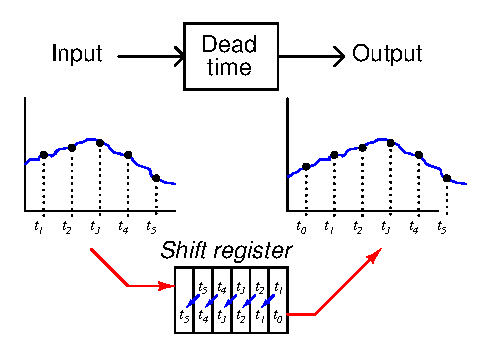
\includegraphics{cont46.eps}$$

\filbreak

Lead and lag functions are also implemented digitally in modern controllers and control systems, but they are actually easier to comprehend in their analog (RC circuit) forms.  The most common way lead and lag functions are found in modern control systems is in combination as the so-called \textit{lead/lag function}, merging both lead and lag characteristics in a single function block (or relay):  \index{Lead/lag function, analog circuit}

% ADD: incorporate discussion of the IEC 61131-3 "delay" function block (for dead time)
% ADD: incorporate a digital lag algorithm into the discussion, a la IEC 61131-3 "lag1" function block, or Shinskey's "Simulating Process Control Loops" book.     xout = xout + k(xin - xout) 

$$\includegraphics{cont47.eps}$$

Each parallel RC subcircuit represents a time constant ($\tau$), one for lead and one for lag.  The overall behavior of the network is determined by the relative magnitudes of these two time constants.  Which ever time constant is larger, determines the overall characteristic of the network.  

\filbreak

If the two time constant values are equal to each other ($\tau_{lead} = \tau_{lag}$), then the circuit performs no dynamic compensation at all, simply passing the input signal to the output with no change except for some attenuation:

$$\includegraphics{cont48.eps}$$

A square wave signal entering this network will exit the network as a square wave.  If the input signal is sinusoidal, the output will also be sinusoidal and in-phase with the input.

\filbreak

If the lag time constant exceeds the lead time constant ($\tau_{lag} > \tau_{lead}$), then the overall behavior of the circuit will be to introduce a first-order lag to the voltage signal:

$$\includegraphics{cont49.eps}$$

A square wave signal entering the network will exit the network as a sawtooth-shaped wave.  A sinusoidal input will emerge sinusoidal, but with a lagging phase shift.  This, in fact, is where the \textit{lag} function gets its name: from the negative (``lagging'') phase shift it imparts to a sinusoidal input.

\filbreak

Conversely, if the lead time constant exceeds the lag time constant ($\tau_{lead} > \tau_{lag}$), then the overall behavior of the circuit will be to introduce a first-order lead to the voltage signal (a step-change voltage input will cause the output to ``spike'' and then settle to a steady-state value):

$$\includegraphics{cont50.eps}$$

A square wave signal entering the network will exit the network with sharp transients on each leading edge.  A sinusoidal input will emerge sinusoidal, but with a leading phase shift.  Not surprisingly, this is where the \textit{lead} function gets its name: from the positive (``leading'') phase shift it imparts to a sinusoidal input.

\filbreak

This exact form of lead/lag circuit finds application in a context far removed from process control: compensation for coaxial cable capacitance in a $\times$10 oscilloscope probe.  Such probes are used to extend the voltage measurement range of standard oscilloscopes, and/or to increase the impedance of the instrument for minimal loading effect on sensitive electronic circuits.  Using a $\times$10 probe, an oscilloscope will display a waveform that is $1 \over 10$ the amplitude of the actual signal, and present ten times the normal impedance to the circuit under test.  \index{$\times$10 oscilloscope probe}  \index{Oscilloscope probe, $\times$10}

If a 9 M$\Omega$ resistor is connected in series with a standard oscilloscope input (having an input impedance of 1 M$\Omega$) to create a 10:1 voltage division ratio, problems will result from the cable capacitance connecting the probe to the oscilloscope input.  What should display as a square-wave input instead looks ``rounded'' by the effect of capacitance in the coaxial cable and at the oscilloscope input:

$$\includegraphics{scope01.eps}$$

The reason for this is signal distortion the combined effect of the 9 M$\Omega$ resistor and the cable's natural capacitance forming an RC network:

\filbreak

$$\includegraphics{scope04.eps}$$

\filbreak

A simple solution to this problem is to build the 10:1 probe with a variable capacitor connected in parallel across the 9 M$\Omega$ resistor.  The combination of the 9 M$\Omega$ resistor and this capacitor creates a lead network to cancel out the effects of the lag caused by the cable capacitance and 1 M$\Omega$ oscilloscope impedance in parallel.  When the capacitor is properly adjusted, the oscilloscope will accurately show the shape of any waveform at the probe tip, including square waves:

$$\includegraphics{scope02.eps}$$

$$\includegraphics{scope05.eps}$$

\filbreak

If we re-draw this compensated probe circuit to show the resistor pair and the capacitor pair both working as 10:1 voltage dividers, it becomes clearer to see how the two divider circuits work in parallel with each other to provide the same 10:1 division ratio \textit{only} if the component ratios are properly proportioned:

$$\includegraphics{scope06.eps}$$

The series resistor pair forms an obvious 10:1 division ratio, with the smaller of the two resistors being in parallel with the oscilloscope input.  The upper resistor, being 9 times larger in resistance value, drops 90\% of the voltage applied to the probe tip.  The series capacitor pair forms a less obvious 10:1 division ratio, with the cable capacitance being the larger of the two.  Recall that the \textit{reactance} of a capacitor to an AC voltage signal is inversely related to capacitance: a larger capacitor will have fewer ohms of reactance for any given frequency according to the formula $X_C = { 1 \over {2 \pi f C}}$.  Thus, the capacitive voltage divider network has the same 10:1 division ratio as the resistive voltage divider network, even though the capacitance ratios may look ``backward'' at first glance.

\filbreak

If the compensation capacitor is adjusted to an excessive value, the probe will \textit{overcompensate} for lag (too much lead), resulting in a ``spiked'' waveform on the oscilloscope display with a perfect square-wave input:

$$\includegraphics{scope03.eps}$$

With the probe's compensating capacitor exhibiting an excessive amount of capacitance, the capacitive voltage divider network has a voltage division ratio \textit{less than} 10:1.  This is why the waveform ``spikes'' on the leading edges: the capacitive divider dominates the network's response in the short term, producing a voltage pulse at the oscilloscope input greater than it should be (divided by some ratio less than 10).  Soon after the leading edge of the square wave passes, the capacitors' effects will wane, leaving the resistors to establish the voltage division ratio on their own.  Since the two resistors have the proper 10:1 ratio, this causes the oscilloscope's signal to ``settle'' to its proper value over time.  Thus, the waveform ``spikes'' too far at each leading edge and then decays to its proper amplitude over time.

While undesirable in the context of oscilloscope probes, this is precisely the effect we desire in a process control \textit{lead} function.  The purpose of a lead/lag function is to provide a signal gain that begins at some initial value, then ``settles'' at another value over time.  This way, sudden changes in the feedforward signal will either be amplified or attenuated for a short duration to compensate for lags in other parts of the control system, while the steady-state gain of the feedforward loop remains at some other value necessary for long-term stability.  For a lag function, the initial gain is less than the final gain; for a lead function, the initial gain exceeds the final gain.  If the lead and lag time constants are set equal to each other, the initial and final gains will likewise be equal, with the function exhibiting a constant gain at all times.

\vskip 10pt

\filbreak

Although lead-lag functions for process control systems may be constructed from analog electronic components, modern systems implement the function arithmetically using digital microprocessors.  A typical time-domain equation describing a digital lead/lag function block's output response ($y$) to an input step-change from zero (0) to magnitude $x$ over time ($t$) is as follows: \index{Lead/lag function, digital implementation}

$$y = x \left(1 + {{{\tau_{lead} - \tau_{lag}} \over \tau_{lag} \> e^{t \over \tau_{lag} }}} \right)$$

As you can see, if the two time constants are set equal to each other ($\tau_{lead} = \tau_{lag}$), the second term inside the parentheses will have a value of zero at all times, reducing the equation to $y = x$.  If the lead time constant exceeds the lag time constant ($\tau_{lead} > \tau_{lag}$), then the fraction will begin with a positive value and decay to zero over time, giving us the ``spike'' response we expect from a lead function.  Conversely, if the lag time constant exceeds the lead ($\tau_{lag} > \tau_{lead}$), the fraction will begin with a negative value at time = 0 (the beginning of the step-change) and decay to zero over time, giving us the ``sawtooth'' response we expect from a lag function.

It should also be evident from an examination of this equation that the ``decay'' time of the lead/lag function is set by the lag time constant ($\tau_{lag}$).  Even if we just need the function to produce a ``lead'' response, we must still properly set $\tau_{lag}$ in order for the lead response to decay at the correct rate for our control system.  The intensity of the lead function (i.e. how far it ``spikes'' when presented with a step-change in input signal) varies with the ratio $\tau_{lead} \over \tau_{lag}$, but the duration of the ``settling'' following that step-change is entirely set by $\tau_{lag}$.

\filbreak

To summarize the behavior of a lead/lag function:

\begin{itemize}
\item If $\tau_{lead} = \tau_{lag}$, the lead/lag function will simply pass the input signal through to the output (no lead or lag action at all)
\item If $\tau_{lead} = 0$, the lead/lag function will provide a pure lag response with a final gain of unity and a time constant of $\tau_{lag}$
\item If $\tau_{lead} = 2 (\tau_{lag})$, the lead/lag function will provide a lead response with an initial gain of 2, a final gain of unity, and a time constant of $\tau_{lag}$
\end{itemize}

$$\includegraphics{cont51.eps}$$













\filbreak
\section{Limit, Selector, and Override controls}

Another category of control strategies involves the use of signal relays or function blocks with the ability to switch between different signal values, or re-direct signals to new pathways.  Such functions are useful when we need a control system to choose between multiple signals of differing value in order to make the best control decisions.

The ``building blocks'' of such control strategies are special relays (or function blocks in a digital control system) shown here:

$$\includegraphics{cont52.eps}$$

\textit{High-select} functions output whichever input signal has the \textit{greatest} value.  \textit{Low-select} functions do just the opposite: output whichever input signal has the \textit{least} value.  ``Greater-than'' and ``Less than'' symbols mark these two selector functions, respectively, and each type may be equipped to receive more than two input signals.  \index{High-select function}  \index{Low-select function}

\filbreak

Sometimes you will see these relays represented in P\&IDs simply by an inequality sign in the middle of the large bubble, rather than off to the side in a square.  You should bear in mind that the location of the input lines has no relationship at all to the direction of the inequality symbol -- e.g., it is not as though a high-select relay looks for the input on the left side to be greater than the input on the right.  Note the examples shown below, complete with sample signal values:

$$\includegraphics{cont53.eps}$$

\filbreak

\textit{High-limit} and \textit{low-limit} functions are similar to high- and low-select functions, but they only receive one input each, and the limit value is a parameter programmed into the function rather than received from another source.  The purpose of these functions is to place a set limit on how high or how low a signal value is allowed to go before being passed on to another portion of the control system.  If the signal value lies within the limit imposed by the function, the input signal value is simply passed on to the output with no modification.  

Like the select functions, limit functions may appear in diagrams with nothing more than the limit symbol inside the bubble, rather than being drawn in a box off to the side:  \index{High-limit function}  \index{Low-limit function}

$$\includegraphics{cont54.eps}$$

\textit{Rate limit} functions place a maximum rate-of-change limit on the input signal, such that the output signal will follow the input signal precisely until and unless the input signal's rate-of-change over time ($dx \over dt$) exceeds the pre-configured limit value.  In that case, the relay still produces a ramping output value, but the rate of that ramp remains fixed at the limit $dx \over dt$ value no matter how fast the input keeps changing.  After the output value ``catches up'' with the input value, the function once again will output a value precisely matching the input unless the input begins to rise or fall at too fast a rate again.  \index{Rate limit function}







\filbreak
\subsection{Limit controls}

A common application for select and limit functions is in \textit{cascade} control strategies, where the output of one controller becomes the setpoint for another.  It is entirely possible for the primary (master) controller to call for a setpoint that is unreasonable or unsafe for the secondary (slave) to attain.  If this possibility exists, it is wise to place a limit function between the two controllers to limit the cascaded setpoint signal.

In the following example, a cascade control system regulates the temperature of molten metal in a furnace, the output of the master (metal temperature) controller becoming the setpoint of the slave (air temperature) controller.  A high limit function limits the maximum value this cascaded setpoint can attain, thereby protecting the refractory brick of the furnace from being exposed to excessive air temperatures:

$$\includegraphics{cont55.eps}$$

It should be noted that although the different functions are drawn as separate bubbles in the P\&ID, it is possible for multiple functions to exist within one physical control device.  In this example, it is possible to find a controller able to perform the functions of both PID control blocks (master and slave) and the high limit function as well.  It is also possible to use a distributed technology such as FOUNDATION Fieldbus to place all control functions inside field instruments, so only three field instruments exist in the loop: the air temperature transmitter, the metal temperature transmitter, and the control valve (with a Fieldbus positioner).

\filbreak

This same control strategy could have been implemented using a low select function block rather than a high limit:

$$\includegraphics{cont56.eps}$$

Here, the low-select function selects whichever signal value is lesser: the setpoint value sent by the master temperature controller, or the maximum air temperature limit value sent by the hand indicating controller (HIC -- sometimes referred to as a \textit{manual loading station}).  \index{Manual loading station}

An advantage of this latter approach over the former might be ease of limit value changes.  With a pre-configured limit value residing in a high-limit function, it might be that only qualified maintenance people have access to changing that value.  If the decision of the operations department is to have the air temperature limit value easily adjusted by anyone, the latter control strategy's use of a manual loading station would be better suited\footnote{I generally suggest keeping such limit values inaccessible to low-level operations personnel.  This is especially true in cases such as this where the presence of a high temperature setpoint limit is intended for the longevity of the equipment.  There is a strong tendency in manufacturing environments to ``push the limits'' of production beyond values considered safe or expedient by the engineers who designed the equipment.  Limits are there for a reason, and should not be altered except by people with full understanding of and full responsibility over the consequences!}.

\vskip 10pt

Another detail to note in this system is the possibility of \textit{integral windup} in the master controller in the event that the high setpoint limit takes effect.  Once the high-limit (or low-select) function secures the slave controller's remote setpoint at a fixed value, the master controller's output is no longer controlling anything: it has become decoupled from the process.  If, when in this state of affairs, the metal temperature is still below setpoint, the master controller's integral action will ``wind up'' the output value over time with absolutely no effect, since the slave controller is no longer following its output signal.  If and when the metal temperature reaches setpoint, the master controller's output will likely be saturated at 100\% due to the time it spent winding up.  This will cause the metal temperature to overshoot setpoint, as a positive error will be required for the master controller's integral action to wind back down from saturation.  \index{Integral windup, limit controls}  \index{Reset windup, limit controls}

\label{override_windup}

\filbreak

A relatively easy solution to this problem is to configure the master controller to stop integral action when the high limit relay engages.  This is easiest to do if the master PID and high limit functions both reside in the same physical controller.  Many digital limit function blocks generate a bit representing the state of that block (whether it is passing the input signal to the output or limiting the signal at the pre-configured value), and some PID function blocks have a boolean input used to disable integral action.  If this is the case with the function blocks comprising the high-limit control strategy, it may be implemented like this:

$$\includegraphics{cont57.eps}$$

\filbreak

Another method used to prevent integral windup is to make use of the \textit{feedback} input available on some PID function blocks.  This is an input used to calculate the integral term of the PID equation.  In the days of pneumatic PID controllers, this option used to be called \textit{external reset}.  Normally connected to the output of the PID block, if connected to the output of the high-limit function it will let the controller know whether or not any attempt to wind up the output is having an effect.  If the output has been de-selected by the high-limit block, integral windup will cease:  \index{External reset, integral control}

$$\includegraphics{cont58.eps}$$

\filbreak

Limit control strategies implemented in FOUNDATION Fieldbus instruments use the same principle, except that the concept of a ``feedback'' signal sending information backwards up the function block chain is an aggressively-applied design philosophy throughout the FOUNDATION Fieldbus standard.  Nearly every function block in the Fieldbus suite provides a ``back calculation'' output, and nearly every function block accepts a ``back calculation'' input from a downstream block.  The ``Control Selector'' (CS) function block specified in the FOUNDATION Fieldbus standard provides the limiting function we need between the master and slave controllers.  The BKCAL\_OUT signal of this selector block connects to the master controller's BKCAL\_IN input, making the master controller aware of its selection status.  If ever the Control Selector function block de-selects the master controller's output, the controller will immediately know to halt integral action:  \index{Back-calculation variable, FOUNDATION Fieldbus function block programming}

$$\includegraphics{cont59.eps}$$

This same ``back calculation'' philosophy -- whereby the PID algorithm is aware of how another function is limiting or over-riding its output -- is also found in some programmable logic controller (PLC) programming conventions.  The Allen-Bradley Logix5000 series of PLCs, for example, provides a \textit{tieback} variable to force the PID function's output to track the overriding function.  When the ``tieback'' variable is properly used, it allows the PID function to bumplessly transition from the ``in-control'' state to the ``overridden'' state.  \index{Tieback variable, Allen-Bradley Logix5000 PLC programming}





\filbreak
\subsection{Selector controls}

In the broadest sense, a ``selector'' control strategy is where one signal is selected from multiple signals in a system to perform a measurement control function.  In the context of this book and this chapter, I will use the term ``selector'' to reference automatic selection among multiple \textit{measurement} or \textit{setpoint} signals.  Selection between multiple \textit{controller output} signals will be explored in the next subsection, under the term ``override'' control.

Perhaps one of the simplest examples of a selector control strategy is where we must select a process variable signal from multiple transmitters.  For example, consider this chemical reactor, where the control system must throttle the flow of coolant to keep the \textit{hottest} measured temperature at setpoint, since the reaction happens to be exothermic (heat-releasing)\footnote{Only the coolant flow control instruments and piping are shown in this diagram, for simplicity.  In a real P\&ID, there would be many more pipes, valves, and other apparatus shown surrounding this process vessel.}:

$$\includegraphics{cont60.eps}$$

The high-select relay (TY-24) sends only the highest temperature signal from the three transmitters to the controller.  The other two temperature transmitter signals are simply ignored.

\vskip 10pt

Another use of selector relays (or function blocks) is for the determination of a \textit{median} process measurement.  This sort of strategy is often used on triple-redundant measurement systems, where three transmitters are installed to measure the exact same process variable, providing a valid measurement even in the event of transmitter failure.  \index{Median signal select}  \index{Redundant transmitters}

\filbreak

The median select function may be implemented one of two ways using high- and low-select function blocks:

$$\includegraphics{cont61.eps}$$

The left-hand selector strategy selects the highest value from each pair of signals (A and B, B and C, A and C), then selects the lowest value of those three primary selections.  The right-hand strategy is exactly opposite -- first selecting the lowest value from each input pair, then selecting the highest of those values -- but it still accomplishes the same function.  Either strategy outputs the \textit{middle} value of the three input signals\footnote{In order to understand how this works, I advise you try a ``thought experiment'' for each function block network whereby you arbitrarily assign three different numerical values for A, B, and C, then see for yourself which of those three values becomes the output value.}.  \index{Thought experiment}  \index{Problem-solving technique: thought experiment}

Although either of these methods of obtaining a median measurement requires four signal selector functions, it is quite common to find function blocks available in control systems ready to perform the median select function all in a single block.  The median-select function is so common to redundant sensor control systems that many control system manufacturers provide it as a standard function unto itself: 

$$\includegraphics{cont85.eps}$$

\filbreak

This is certainly true in the FOUNDATION Fieldbus standard, where two standardized function blocks are capable of this function, the CS (Control Selector) and the ISEL (Input Selector) blocks:  \index{ISEL Fieldbus function block}  \index{CS Fieldbus function block}

$$\includegraphics{cont62.eps}$$

Of these two Fieldbus function blocks, the latter (ISEL) is expressly designed for selecting transmitter signals, whereas the former (CS) is best suited for selecting controller outputs with its ``back calculation'' facilities designed to modify the response of all de-selected controllers.  Using the terminology of this book section, the ISEL function block is best suited for \textit{selector} strategies, while the CS function block is ideal for \textit{limit} and \textit{override} strategies (discussed in the next section).  \index{Back-calculation variable, FOUNDATION Fieldbus function block programming}

If receiving three ``good'' inputs, the ISEL function block will output the middle (median) value of the three.  If one of the inputs carries a ``bad'' status\footnote{In FOUNDATION Fieldbus, each and every signal path not only carries the signal value, but also a ``status'' flag declaring it to be ``Good,'' ``Bad,'' or ``Uncertain.''  This status value gets propagated down the entire chain of connected function blocks, to alert dependent blocks of a possible signal integrity problem if one were to occur.}, the ISEL block outputs the averaged value of the remaining two (good) inputs.  Note how this function block also possesses individual ``disable'' inputs, giving external boolean (on/off) signals the ability to disable any one of the transmitter inputs to this block.  Thus, the ISEL function block may be configured to de-select a particular transmitter input based on some programmed condition other than internal diagnostics.

If receiving four ``good'' inputs, the ISEL function block normally outputs the average value of the two middle (median) signal values.  If one of the four inputs becomes ``bad'' is disabled, the block behaves as a normal three-input median select.

\vskip 10pt

A general design principle for redundant transmitters is that you \textit{never} install exactly two transmitters to measure the same process variable.  Instead, you should install three (minimum).  The problem with having two transmitters is a lack of information for ``voting'' if the two transmitters happen to disagree.  In a three-transmitter system, the function blocks may select the median signal value, or average the ``best 2 out of 3.''  If there are just two transmitters installed, and they do not substantially agree with one another, it is anyone's guess which one should be trusted\footnote{This principle holds true even for systems with no function blocks ``voting'' between the redundant transmitters.  Perhaps the installation consists of two transmitters with remote indications for a human operator to view.  If the two displays substantially disagree, which one should the operator trust?  A set of \textit{three} indicators would be much better, providing the operator with enough information to make an intelligent decision on which display(s) to trust.}.  \index{Voting system}

\vskip 10pt

\filbreak

A classic example of selectors in industrial control systems is that of a \textit{cross-limited ratio control} strategy for air/fuel mixture applications.  Before we explore the use of selector functions in such a strategy, we will begin by analyzing a simplified version of that strategy, where we control air and fuel flows to a precise ratio with no selector action at all:

$$\includegraphics{cont71.eps}$$

Here, the fuel flow controller receives its setpoint directly from the firing command signal, which may originate from a human operator's manual control or from the output of a temperature controller regulating temperature of the combustion-heated process.  The air flow controller receives its setpoint from the fuel flow transmitter, with the calibrations of the air and fuel flow transmitters being appropriate to establish the proper air:fuel flow ratio when the transmitters register equally.  From the perspective of the air flow controller, fuel flow is the \textit{wild} flow while air flow is the \textit{captive} flow.  \index{Wild flow}  \index{Captive flow}

There is a problem with this control system that may not be evident upon first inspection: the air:fuel ratio will tend to vary as the firing command signal increases or decreases in value over time.  This is true even if the controllers are well-tuned and the air:fuel ratio remains well-controlled under steady-state conditions.  The reason for this is linked to the roles of ``wild'' and ``captive'' flows, fuel and air flow respectively.  Since the air flow controller receives its setpoint from the fuel flow transmitter, changes in air flow will always \textit{lag} behind changes in fuel flow.  

This sort of problem can be difficult to understand because it involves changes in multiple variables over time.  A useful problem-solving technique to apply here is a ``thought experiment,'' coupled with a time-based graph to display the results.  Our thought experiment consists of imagining what would happen if the firing command signal were to \textit{suddenly} jump in value, then sketching the results on a graph.

\filbreak

If the firing command signal suddenly increases, the fuel flow controller responds by opening up the fuel valve, which after a slight delay results in increased fuel flow to the burner.  This increased fuel flow signal gets sent to the setpoint input of the air flow controller, which in turn opens up the air valve to increase air flow proportionately.  If the firing command signal suddenly decreased, the same changes in flow would occur in reverse direction but in the same chronological sequence, since the fuel flow change still ``leads'' the subsequent air flow change:  \index{Thought experiment}  \index{Problem-solving technique: thought experiment}

$$\includegraphics{cont72.eps}$$

Inevitable delays in controller response, valve response, and flow transmitter response conspire to upset the air:fuel ratio during the times immediately following a step-change in firing command signal.  When the firing command steps up, the fuel flow increases before the air flow, resulting in a short time when the burner runs ``rich'' (too much fuel, not enough air).  When the firing command steps down, the fuel flow decreases before the air flow, resulting in a short time when the burner runs ``lean'' (too much air, not enough fuel).  The scenario problem is dangerous because it may result in an explosion if an accumulation of unburnt fuel collects in a pocket of the combustion chamber and then ignites.  The second scenario is generally not a problem unless the flame burns \textit{so} lean that it risks blowing out.

\vskip 10pt

The solution to this vexing problem is to re-configure the control scheme so that the air flow controller ``takes the lead'' whenever the firing command signal rises, and that the fuel flow controller ``takes the lead'' whenever the firing command signal falls.  This way, any upsets in air:fuel ratio resulting from changes in firing command will always err on the side of a lean burn rather than a rich burn.

\filbreak

We may implement precisely this strategy by adding some signal selector functions to our ratio control system.  The ratio is now \textit{cross-limited}, where both measured flow rates serve as limiting variables to each other to ensure the air:fuel ratio can never be too rich:

$$\includegraphics{cont74.eps}$$

Now, the air flow controller receives its setpoint either directly from the firing command signal or from the fuel flow transmitter, whichever signal is \textit{greater} in value.  The fuel flow controller receives its setpoint either directly from the firing command signal or from the air flow transmitter, whichever signal is \textit{least} in value.  Thus, the air flow controller ``takes the lead'' and makes fuel flow the ``captive'' variable when the firing command signal rises.  Conversely, the fuel flow controller ``takes the lead'' and makes air flow the ``captive'' variable when the firing command signal falls.  Instead of having the roles of ``wild'' and ``captive'' flows permanently assigned, these roles switch depending on which way the firing command signal changes.

\filbreak

Examining the response of this cross-limited system to sudden changes in firing command signal, we see how the air flow controller takes the lead whenever the firing rate signal increases, and how the fuel flow controller takes the lead whenever the firing rate signal decreases:

$$\includegraphics{cont84.eps}$$

In both transient scenarios, the mixture runs lean (safe) rather than rich (dangerous).  Of course, care must be taken to ensure the firing rate signal never steps up or down so quickly that the flame runs lean enough to blow out (i.e. the mixture becomes much too lean during a transient ``step-change'' of the firing rate signal).  If this is a problem, we may fix it by installing \textit{rate-limiting} functions in the firing command signal path, so that the firing command signal can never rise or fall too rapidly.

\filbreak

A realistic cross-limited ratio control system also incorporates a means to adjust the air:fuel ratio without having to re-range the air and/or fuel flow transmitters.  Such ratio adjustment may be achieved by the insertion of a ``multiplying'' function between one of the selectors and a controller setpoint, plus a ``dividing'' function to return that scaled flow to a normalized value for cross-limiting.

The complete control strategy looks something like this, complete with cross-limiting of air and fuel flows, rate-limiting of the firing command signal, and adjustable air:fuel ratio:

$$\includegraphics{cont73.eps}$$








\filbreak
\subsection{Override controls}

An ``override'' control strategy involves a selection between two or more controller \textit{output} signals, where only one controller at a time gets the opportunity to exert control over a process.  All other ``de-selected'' controllers are thus \textit{overridden} by the selected controller.

\vskip 10pt

The general concept of override control is easily understood by appeal to a human example.  Cargo truck drivers must monitor and make control decisions on a wide number of variables, including diesel engine operating parameters and road rules.  A truck driver needs to keep a close watch on the exhaust gas temperature of the truck engine: a leading indicator of impending engine damage (if exhaust temperature exceeds a pre-determined limit established by the engine manufacturer).  The same truck driver must also drive as fast as the law will allow on any given road in order to minimize shipping time and thereby maximize the amount of cargo transported over long periods of time.  These two goals may become mutually exclusive when hauling heavy cargo loads up steep inclines, such as when ascending a mountain pass.  The goal of avoiding engine damage necessarily overrides the goal of maintaining legal road speed in such conditions.

Imagine a diesel truck driver maintaining the legal speed limit on a highway, occasionally glancing at the EGT (Exhaust Gas Temperature) indicator in the instrument panel.  Under normal operating conditions, the EGT should be well below the danger threshold for the engine.  However, after pulling a full load up a mountain pass and noticing the EGT approach the high operating limit, the truck driver makes the decision to regulate the engine's power based on EGT rather than road speed.  In other words, the legal speed limit is no longer the ``setpoint'' to control to, and EGT now is.

If we were to model the truck driver's decision-making processes in industrial instrumentation terms, it would look something like this:

$$\includegraphics{cont83.eps}$$

Which ever control decision calls for the least engine power output, ``wins the vote'' to control the engine's power. 

\filbreak

As is the case with limit and selector control strategies, a ``select'' function is used to choose one signal from multiple signals.  The difference here is that the signals being selected are both \textit{controller outputs} rather than transmitter (measurement) or setpoint signals.  Both controllers are still active, but only one at a time will have any actual control over the process.

This model maps well to the truck driver analogy.  Despite having ``overridden'' the goal of maintaining legal road speed in favor of maintaining a safe engine exhaust temperature, the driver is still thinking about road speed.  In fact, if the driver happens to be behind schedule, you can be absolutely sure the goal of maintaining the highway speed limit has not been forgotten!  In fact, the driver may become impatient as the long incline wears on, eager to make up lost time as soon as the opportunity allows.  This is a potential problem for all override control systems: making sure the de-selected controller does not ``wind up'' (with integral action still active) while it has no control over the process.

\vskip 10pt

An municipal example of override control is seen in this water pumping system, where a water pump is driven by a variable-speed\footnote{In most applications this takes the form of an AC induction motor receiving power from a \textit{Variable Frequency Drive} or \textit{VFD}.  Since the rotational speed of an induction motor is a function of frequency, the VFD achieves motor speed control by electronically converting the fixed-frequency line power into variable-frequency power to drive the motor.} electric motor to draw water from a well and provide constant water pressure to a customer:  \index{Variable-frequency drive}  \index{VFD}

$$\includegraphics{cont65.eps}$$

Incidentally, this is an excellent application for a variable-speed motor as the final control element rather than a control valve.  Reducing pump speed in low-flow conditions will save a lot of energy over time compared to the energy that would be wasted by a constant-speed pump and control valve.

A potential problem with this system is the pump running ``dry'' if the water level in the well gets too low, as might happen during summer months when rainfall is low and customer demand is high.  If the pump runs for too long with no water passing through it, the seals will become damaged.  This will necessitate a complete shut-down and costly rebuild of the pump, right at the time customers need it the most.

\filbreak

One solution to this problem would be to install a level switch in the well, sensing water level and shutting off the electric motor driving the pump if the water level ever gets too low:

$$\includegraphics{cont64.eps}$$

This may be considered a kind of ``override'' strategy, because the low-level switch over-rides the pressure controller's command for the pump to turn.  It is also a crude solution to the problem, for while it protects the pump from damage, it does so at the cost of completely shutting off water to customers.  One way to describe this control strategy would be to call it a \textit{hard override} system, suggesting the uncompromising action it will take to protect the pump.  \index{Hard override}  \index{Override, hard}

\filbreak

A better solution to the dilemma would be to have the pump merely slow down as the well water level approaches a low-level condition.  This way at least the pump could be kept running (and some amount of pressure maintained), decreasing demand on the well while maintaining curtailed service to customers and still protecting the pump from dry-running.  This would be termed a \textit{soft override} system.  \index{Soft override}  \index{Override, soft}

We may create just such a control strategy by replacing the well water level switch with a level \textit{transmitter}, connecting the level transmitter to a level controller, and using a low-select relay or function block to select the lowest-valued output between the pressure and level controllers.  The level controller's setpoint will be set at some low level above the acceptable limit for continuous pump operation:

$$\includegraphics{cont63.eps}$$

If ever the well's water level goes below this setpoint, the level controller will command the pump to slow down, even if the pressure controller is calling for a higher speed.  The level controller will have \textit{overridden} the pressure controller, prioritizing pump longevity over customer demand.

Bear in mind that the concept of a low-level switch completely shutting off the pump is not an entirely bad idea.  In fact, it might be prudent to integrate such a ``hard'' shutdown control in the override control system, just in case something goes wrong with the level controller (e.g. an improperly adjusted setpoint or poor tuning) or the low-select function.  

\filbreak

With two layers of safety control for the pump, this system provides both a ``soft constraint'' providing moderated action and a ``hard constraint'' providing aggressive action to protect the pump from dry operation:  \index{Soft constraint}  \index{Hard constraint}  \index{Constraint, hard versus soft}  \index{Override, hard versus soft}

$$\includegraphics{cont66.eps}$$

In order that these two levels of pump protection work in the proper order, the level controller's (LC) setpoint needs to be set to a higher value than the low level alarm's (LAL) trip point.

\vskip 10pt

A very important consideration for any override control strategy is how to manage integral windup.  Any time a controller with any integral (reset) action at all is de-selected by the selector function, the integral term of the controller will have the tendency to wind up (or wind down) over time.  With the output of that controller de-coupled from the final control element, it can have no effect on the process variable.  Thus, integral control action -- the purpose of which being to constantly drive the output signal in the direction necessary to achieve equality between process variable and setpoint -- will work in vain to eliminate an error it cannot influence.  If and when control is handed back to that controller, the integral action will have to spend time ``winding'' the other way to un-do what it did while it was de-selected.  \index{Integral windup, override controls}  \index{Reset windup, override controls}

Thus, override controls demand some form of integral windup limits that engage when a controller is de-selected.  Methods of accomplishing this function are discussed in an earlier section on limit controls (section \ref{override_windup} beginning on page \pageref{override_windup}).

% ADD: (Override) -- flow control with tank level limit
% ADD: (Override) -- compressor speed control (Shinskey)











%\filbreak
%\section{Adaptive gain control}

% ADD: water chlorination controls (gain adapts with water flow rate)












%\filbreak
%\section{Decoupling controls}

% ADD: furnace draft/firing controls








%\filbreak
%\section{Analog signal relays}

% In the days when pneumatic technology dominated industrial instrumentation and control system design, it was standard practice to implement control strategies such as ratio, dynamic compensation, selector, and override using special \textit{signal relay} devices.  These pneumatic devices performed the signal processing necessary to alter and select signal values between transmitters, controllers, and final control elements.

% Later, when analog electronic circuit development reached a point robust enough for critical control applications, these same functions were implemented in semiconductor form, the signals being voltage and current instead of pneumatic (air) pressure.

% This section explores some of the technology once commonly used to implement mathematical and selection functions in control systems.  Although these signal ``relays'' have all but been replaced by algorithms executed in digital computers, some examples may still be found in industrial use at the time of this writing (2009).

% REFER TO PC191 FOXBORO-ECKARDT COMPUTING RELAYS CATALOG





%\filbreak
%\subsection{Pneumatic signal boosters}







%\filbreak
%\subsection{Low-select and high-select relays}







%\filbreak
%\subsection{Lead and lag relays}







%\filbreak
%\subsection{Special function relays}










\filbreak
\section{Techniques for analyzing control strategies}

Control strategies such as cascade, ratio, feedforward, and those containing limit and selector functions can be quite daunting to analyze, especially for students new to the subject.  As a teacher, I have seen first-hand where students tend to get confused on these topics, and have seen how certain problem-solving techniques work well to overcome these conceptual barriers.  This section explores some of these techniques and the reasons why they work.



\filbreak
\subsection{Explicitly denoting controller actions}

The direction of action for a loop controller -- either \textit{direct} or \textit{reverse} -- at first seems like a very simple concept.  It certainly is fundamental to the comprehension of any control strategy containing PID loop controllers, but this seemingly simple concept harbors an easy-to-overlook fact causing much confusion for students as they begin to analyze any control strategy where a loop controller receives a remote setpoint signal from some other device, most notably in cascade and ratio control strategies.  \index{Direct-acting controller}  \index{Reverse-acting controller}  \index{Action, controller}  \index{Controller action, direct vs. reverse}

A \textit{direct-acting} loop controller is defined as one where the output signal increases as the process variable signal increases.  A \textit{reverse-acting} controller is defined as one where the output signal decreases as the process variable signal increases.  Both types of action are shown here:

$$\includegraphics{cont88.eps}$$

\filbreak

Let us apply this concept to a realistic application, in this case the control of temperature in a steam-heated chemical reactor vessel:

$$\includegraphics{cont89.eps}$$

As the reactor vessel's temperature increases, we need the temperature controller (TIC) to reduce the amount of hot steam entering the jacket in order to stabilize that temperature.  Since the steam control valve is air-to-open (ATO), this means we need the controller to output a \textit{decreasing} signal as the process variable (temperature) signal increases.  This, by definition, is a \textit{reverse-acting} controller.  This example also showcases the utility of the problem-solving technique known as a ``thought experiment,'' whereby we imagine a certain condition changing (in this case, the reactor temperature increasing) and then we mentally model the desired response of the system (in this case, closing the steam valve) in order to determine the necessary controller action. \index{Thought experiment}  \index{Problem-solving technique: thought experiment}

So far, this example poses no confusion.  But suppose we were to perform another thought experiment, this time supposing the \textit{setpoint} signal increases rather than the reactor temperature increases.  How will the controller respond now?

Many students will conclude that the controller's output signal will once again decrease, because we have determined this controller's action to be \textit{reverse}, and ``reverse'' implies the output will go the opposite direction as the input.  However, this is not the case: the controller output will actually \textit{increase} if its setpoint signal is increased.  This, in fact, is precisely how any reverse-acting controller should respond to an increase in setpoint.

\filbreak

The reason for this is evident if we take a close look at the characteristic equation for a reverse-acting proportional controller.  Note how the gain is multiplied by the difference between setpoint and process variable.  Note how the process variable has a negative sign in front of it, while setpoint does not.

$$\includegraphics{cont90.eps}$$

An increase in process variable (PV) causes the quantity inside the parentheses to become more negative, or less positive, causing the output to decrease toward 0\%.  Conversely, an increase in setpoint (SP) causes the quantity inside the parentheses to become more positive, causing the output to increase toward 100\%.  This is precisely how any loop controller should respond: with the setpoint having the opposite effect of the process variable, because those two quantities are always being \textit{subtracted} from one another in the proportional controller's equation.

Where students get confused is the single label of either ``direct'' or ``reverse'' describing a controller's action.  We define a controller as being either ``direct-acting'' or ``reverse-acting'' based on how it responds to changes in process variable, but it is easy to overlook the fact that the controller's setpoint input must necessarily have the \textit{opposite} effect.  What we really need is a way to more clearly denote the respective actions of a controller's two inputs than a single word.

\filbreak

Thankfully, such a convention already exists in the field of electronics\footnote{Some differential pressure transmitter manufacturers, such as Bailey, apply the same convention to denote the actions of a DP transmitter's two pressure ports: using a ``+'' label to represent direct action (i.e. increasing pressure at this port drives the output signal up) and a ``$-$'' symbol to represent reverse action (i.e. increasing pressure at this port drives the output signal down).}, where we must denote the ``actions'' of an operational amplifier's two inputs.  In the case of an opamp, one input has a direct effect on the output (i.e. a change in signal at that input drives the output the same direction) while the other has a reverse effect on the output (i.e. a change in signal at that input drives the output in the opposite direction).  Instead of calling these inputs ``direct'' and ``reverse'', however, they are conventionally denoted as \textit{noninverting} and \textit{inverting}, respectively.  If we draw a proportional controller as though it were an opamp, we may clearly denote the actions of both inputs in this manner:

$$\includegraphics{cont91.eps}$$

I strongly recommend students label the loop controllers in any complex control strategy in the same manner, with ``+'' and ``$-$'' labels next to the PV and SP inputs for each controller, in order to unambiguously represent the effects of each signal on a controller's output.  This will be far more informative, and far less confusing, than merely labeling each controller with the word ``direct'' or ``reverse''.

\filbreak

Let us return to our example of the steam-heated reactor to apply this technique, labeling the reverse-acting controller's process variable input with a ``$-$'' symbol and its setpoint input with a ``+'' symbol:

$$\includegraphics{cont92.eps}$$

With these labels in place we can see clearly how an increase in temperature going into the ``$-$'' (inverting) input of the temperature controller will drive the valve signal down, counter-acting the change in temperature and thereby stabilizing it.  Likewise, we can see clearly how an increase in setpoint going into the ``+'' (noninverting) input of the temperature controller will drive the valve signal up, sending more steam to the reactor to achieve a greater temperature.

\vskip 10pt

While this technique of labeling the PV and SP inputs of a loop controller as though it were an operational amplifier is helpful in single-loop controller systems, it is incredibly valuable when analyzing more complex control strategies where the setpoint to a controller is a live signal rather than a static value set by a human operator.  In fact, it is for this very reason that many students do not begin to have trouble with this concept until they begin to study cascade control, where one controller provides a live (``remote'') setpoint value to another controller.  Up until that point in their study, they never rarely had to consider the effects of a setpoint change on a control system because the setpoint value for a single-loop controller is usually static.

\filbreak

Let us modify our steam-heated reactor control system to include a cascade strategy, where the temperature controller drives a setpoint signal to a ``slave'' steam flow controller:

$$\includegraphics{cont93.eps}$$

In order to determine the proper actions for each controller in this system, it is wise to begin with the slave controller (FIC), since the master controller (TIC) depends on the slave controller being properly configured in order to do its job properly.  Just as we would first tune the slave controller in a cascade system prior to tuning the master controller, we should first determine the correct action for the slave controller prior to determining the correct action for the master controller.

\filbreak

Once again we may apply a ``thought experiment'' to this system in order to choose the appropriate slave controller action.  If we imagine the steam flow rate suddenly increasing, we know we need the control valve to close off in order to counter-act this change.  Since the valve is still air-to-open, this requires a decrease in the output signal from the FIC.  Thus, the FIC must be reverse-acting.  We shall denote this with a ``$-$'' label next to the process variable (PV) input, and a ``+'' label next to the remote setpoint (RSP) input:

$$\includegraphics{cont94.eps}$$

\filbreak

Now that we know the slave controller must be reverse-acting, we may choose the action of the master controller.  Applying another ``thought experiment'' to this system, we may imagine the reactor temperature suddenly increasing.  If this were to happen, we know we would need the control valve to close off in order to counter-act this change: sending less steam to a reactor that is getting too hot.  Since the valve is air-to-open, this requires a decrease in the output signal from the FIC.  Following the signal path backwards from the control valve to the FIC to the TIC, we can see that the TIC must output a decreasing signal to the FIC, calling for less steam flow.  A decreasing output signal at the TIC enters the FIC's noninverting (``+'') input, causing the FIC output signal to also decrease.  Thus, we need the TIC to be reverse-acting as well.  We shall denote this with a ``$-$'' label next to the process variable (PV) input, and a ``+'' label next to the local setpoint (LSP) input:

$$\includegraphics{cont95.eps}$$

With these unambiguous labels in place at each controller's inputs, we are well-prepared to qualitatively analyze the response of this cascade control system to process upsets, to instrument failure scenarios, or to any other change.  No longer will we be led astray by the singular label of ``reverse-acting'', but instead will properly recognize the different directions of action associated with each input signal to each controller.









\filbreak
\subsection{Determining the design purpose of override controls}

Override control strategies are a source of much confusion for students first learning the concept.  Perhaps the most fundamental question students find difficult to answer when faced with an override strategy is how to determine the intended purpose for that strategy if no explanation is given.

\vskip 10pt

Take for example this surge tank level/flow control system.  While it may be obvious that the flow controller is there for the purpose of regulating flow out of the tank, it is not so clear what the two level controllers are doing, or what purposes are served by the two selector functions:

$$\includegraphics{cont96.eps}$$

A good starting point in our analysis is to first determine the proper directions of action for each controller.  This is wise because the selector functions perform their tasks based on the relative values of the controller output signals: controllers become selected or de-selected on the basis of their output signals being greater or less than some other signal.  Therefore, before we may be able to determine the purpose of a selector function, we must know how the loop controller feeding that selector function is supposed to react to process conditions.  Once we have determined each controller's proper action, we may then interpret each selector's function in light of what process conditions will cause a particular controller to become selected.

\filbreak

When choosing the proper action for each controller, we must consider each controller in this system -- one at a time -- as though it were the one being selected.  In other words, we may give ourselves license to ignore the selector functions and just concentrate for the time being on how each controller needs to act in order to do its job when selected.  Looking at the system from this perspective, we see that each level controller (when selected) acts as a master to the flow (slave) controller.  Thus, what we have here is a cascade level/flow control system, with two master controllers selected on the basis of their output signals.

The flow controller (FIC) needs to be reverse-acting, because in order to counter-act an increase in flow rate it must close off the valve (i.e. decreasing output with increasing input = reverse action).  Each level controller needs to be direct-acting, because in order to counter-act an increase in level it must call for more flow exiting the tank (i.e. increasing output with increasing input = direct action).  Denoting these actions using ``+'' and ``$-$'' labels at each PV and SP input line:

$$\includegraphics{cont97.eps}$$

Only now are we prepared to analyze the purpose of each selector function.  Let's begin with the low-select first.  It selects the lowest of two values, either a fixed value of 50\% or the output of the level controller with the 10\% setpoint.  Since we know this level controller is direct-acting, we may conclude that it will be selected if it sees a \textit{low level} at its PV input.  More specifically, it will be surely be selected if the measured tank level drops significantly below the setpoint value of 10\%.  Thus, we may conclude that the purpose of this level controller is to take over control if the tank level reaches or drops below the 10\% mark.

Next, let us analyze the purpose of the other level controller (connected to the high-select function).  Since the high-select function will select this level controller only if its output signal exceeds the signal passed on by the low-select function, and we know that this controller is direct-acting, we may conclude that it will be selected if it sees a \textit{high level} at its PV input.  More specifically, it will surely be selected if the measured tank level rises significantly above the setpoint value of 90\%.  Thus, we may conclude that the purpose of this level controller is to take over control if the tank level reaches or exceeds the 90\% mark.

If neither level controller is selected, the signal that gets passed on to the flow controller as a remote setpoint is the 50\% fixed signal entering on the left-hand side of the low-select function.  Thus, the flow controller tries to maintain a steady flow rate of 50\% in the event neither level controller is selected.

\vskip 10pt

Putting all these pieces together, we may conclude that the purpose of this surge tank control system is to maintain as steady a flow rate as possible out of the tank (and on to some other process), letting the liquid level inside the tank rise and fall significantly before any action is taken to change the flow rate.  Only if the level drops below 10\% will the flow rate be reduced, and only if the level rises above 90\% will the flow rate be increased.  Otherwise, the flow rate will hold steady at 50\%.

\vskip 10pt

To summarize, the recommended technique for analyzing the purpose of an override control system is as follows:

\begin{itemize}
\item First, determine the necessary actions of each controller (assume the selector functions are absent, and each controller gets its turn controlling the process).
\item Identify the type of selection (high or low) implemented by each selector function.
\item Based on the type of selection and the action of the controller, identify what process condition will cause that controller to become selected.  \textit{This is the condition the controller exists to regulate.}
\end{itemize}












%\filbreak
%\section{Transfer function analysis}

%A powerful analytical technique used in control engineering describes elements within process control loops in mathematical terms of growing/decaying sinusoidal quantities.  As detailed in a previous section of this book (section \ref{s_variable} beginning on page \pageref{s_variable}), the $s$ variable is a concise way to represent sinusoidal signals exponentially growing or decaying over time: $s$ is a \textit{complex number} with a ``real'' part ($\sigma$) describing the growth/decay rate of the signal and an ``imaginary'' part ($j \omega$) describing the frequency of the signal:

%$$s = \sigma + j \omega$$

%\noindent
%Where,

%$s$ = Complex growth/decay rate and frequency (sec$^{-1}$)

%$\sigma$ = Signal growth/decay rate (time constants per second, or sec$^{-1}$)

%$j$ = Imaginary operator (equal to $\sqrt{-1}$)

%$\omega$ = Signal frequency (radians per second, or sec$^{-1}$)

%\vskip 10pt

%$s$ translates to a wave by Euler's Relation\footnote{Leonhard Euler proved that $e^{j \theta} = \cos \theta + j \sin \theta$, where $\theta$ is any arbitrary angle.  Instead of using $\theta$ to describe the phasor's angle, engineers use the product $\omega t$ which is the angular velocity (frequency) of the signal multiplied by time, but it means the same thing.} which tells us when $e$ is raised to an imaginary power it describes a phasor for a sinusoidal wave.  A real-number exponent of $e$ describes a growth or decay rate.  Combining the real and imaginary portions of $s$ together into one exponential function allows us to describe both the growth/decay rate and the frequency for any sinusoidal signal in one concise expression:  \index{Euler, Leonhard}

%$$Ae^{st} = Ae^{(\sigma + j\omega)t} = Ae^{\sigma t} e^{j \omega t}$$

%\noindent
%Where,

%$A$ = Initial amplitude of the sinusoid (e.g. volts, amps) at time $t = 0$ (arbitrary units)

%$s$ = Complex growth/decay rate and frequency

%$\sigma$ = $1 \over \tau$ = Real growth/decay rate (time constants per second, or sec$^{-1}$)

%$j \omega$ = Imaginary frequency (radians per second, or sec$^{-1}$)

%$t$ = Time (seconds)

%\vskip 10pt

%Separating the expression $Ae^{\sigma t} e^{j \omega t}$ into three parts -- $A$, $e^{\sigma t}$, and $e^{j \omega t}$ -- we get a complete description of a rotating phasor:

%\vskip 10pt

%$A$ = Initial amplitude of the phasor ($t = 0$)

%$e^{\sigma t}$ = How much the phasor's magnitude has grown ($\sigma > 0$) or decayed ($\sigma < 0$) at time $t$

%$e^{j \omega t}$ = Unit phasor (length = 1) at time $t$

%\vskip 10pt

%\filbreak

%If we set $\omega$ at some constant value and experiment with different values of $\sigma$, we can see the effect $\sigma$ has on the shape of the wave over time:

%$$\includegraphics{complex_11.eps}$$

%If we set $\sigma$ at zero and experiment with different values\footnote{One value of $\omega$ not shown in this three-panel graphic comparison is a \textit{negative} frequency.  This is actually not as profound as it may seem at first.  All a negative value of $\omega$ will do is ensure that the phasor will rotate in the opposite direction (clockwise, instead of counter-clockwise as phasor rotation is conventionally defined).  The real portion of the sinusoid will be identical, tracing the same cosine-wave plot over time.  Only the imaginary portion of the sinusoid will be different, as $j \sin - \theta = - j \sin \theta$.} of $\omega$, we can see the effect $\omega$ has on the shape of the wave over time:

%$$\includegraphics{complex_27.eps}$$

%$Ae^{st}$ is an example of a \textit{time-domain} function because we customarily set $s$ to some constant value and let time ($t$) be the independent variable.  The resulting function is graphed with time on the horizontal axis (the ``domain'' of the graph).  However, it is possible to write mathematical expressions not containing $t$ at all, but only $s$ as the independent variable.  In that case, the function is called an \textit{$s$-domain} function.  Since $s$ is a complex variable with both real and imaginary parts, the graph of an $s$-domain function is best plotted as a three-dimensional surface, where $s$ is specified by real and imaginary coordinates on a two-dimensional \textit{plane}.  \index{$s$ domain}  \index{Time domain}

%\filbreak

%A mathematical function of $s$ for any process system, therefore, describes that system's response to stimuli having various rates of growth or decay and various frequencies of oscillation.  The general idea of the $s$ variable is that it becomes a frame of reference for describing the behavior of any linear system.  Having a mathematical model of a system written in terms of $s$ yields certain insights into the behavior of that system which would be much more difficult to see strictly from the perspective of time ($t$).  Consider the following resistor-capacitor circuit as a ``process'' to analyze in this manner:

%$$\includegraphics{complex_26.eps}$$

%An electronic technician would probably be familiar with following equation describing the time-domain behavior of this circuit, assuming $V_{in}$ was a DC voltage suddenly applied across the input terminals:

%$$V_{out} = V_{in} \left(1 - e^{-t / RC} \right)$$

%By plugging in different values for $V_{in}$ and $t$, one could use this formula to compute the output voltage of the circuit at any given point in time following the application of $V_{in}$.

%\vskip 10pt

%An electrical engineer, however, could also describe this same circuit's behavior in the $s$ domain:

%$$V_{out}(s) = V_{in}(s) \left({1 \over 1 + sRC} \right)$$

%By plugging in different values for $s$, one could use this formula compute the magnitude and phase shift of the output voltage for any given input voltage growth/decay rate and frequency.

%\vskip 10pt

%It should be noted that $s$-domain analysis is a general tool applicable to any linear system, not just to electrical circuits.  For the context of this chapter, the real and imaginary parts of $s$ hold practical information regarding control system performance: the real part of $s$ tells us whether a control loop will stabilize at a particular point ($\sigma < 0$) or ``run away'' ($\sigma > 0$), while the imaginary part of $s$ tells us the frequency at which a control loop will tend to oscillate.  These are both extremely important parameters in control system design, which is why $s$-domain analysis is important for control system engineers to learn.

%As a case in point, the resistor-capacitor circuit we just looked at is an example of a \textit{first order lag system}.  Many physical processes exhibit the same behavior and therefore may be modeled by similar time-domain and $s$-domain functions.

%\filbreak

%Building on the concept of using $s$ to describe sinusoidal signals, engineers also describe the output/input \textit{ratios} of systems and system elements in terms of $s$.  These ratios are called \textit{transfer functions} and are analogous to the \textit{gain} ratios of electronic circuit networks.  For the simple electrical circuit shown above, the transfer function is as follows:

%$$\hbox{Transfer function} = {V_{out}(s) \over V_{in}(s)} = {1 \over 1 + sRC}$$

%If we replace the electrically-specific quantities of ``resistance'' ($R$) and ``capacitance'' ($C$) with the more general quantity of ``time constant'' or ``lag time'' ($\tau$), we may re-write the transfer function in terms applicable to \textit{any} first-order lag system:

%$$\hbox{Transfer function} = {\hbox{Output}(s) \over \hbox{Input}(s)} = {1 \over 1 + s \tau}$$

%\vskip 10pt


%%%% To be continued . . .









\filbreak
\section{Review of fundamental principles}

Shown here is a partial listing of principles applied in the subject matter of this chapter, given for the purpose of expanding the reader's view of this chapter's concepts and of their general inter-relationships with concepts elsewhere in the book.  Your abilities as a problem-solver and as a life-long learner will be greatly enhanced by mastering the applications of these principles to a wide variety of topics, the more varied the better.

\begin{itemize}
%\item \textbf{$s$ variable}: a complex variable mathematically defined as $s = \sigma + j \omega$.  Used to describe a sinusoidal wave with a given growth or decay rate ($\sigma$) and frequency ($\omega$).  Relevant to process control stability: $\omega$ describes the frequency that a loop will tend to oscillate at, while $\sigma$ determines whether the loop will stabilize following a disturbance ($\sigma < 0$) or ``run away'' following a disturbance ($\sigma > 0$).
%\item \textbf{Euler's Relation}: a mathematical relationship between complex numbers and sine/cosine functions.  For any angle $\theta$, Euler's Relation tells us that $e^{j \theta} = \cos \theta + j \sin \theta$.  Relevant to the $s$ variable, where $e^{st}$ describes a sinusoidal wave with a specified growth/decay rate ($\sigma$) and frequency ($\omega$).
%\item \textbf{Laplace transform}: a mathematical technique for translating a time-domain function into an $s$-domain function.  Relevant to process characteristics and feedback control loops, where the laws of physics and chemistry often provide differential equations characterizing portions of the system, but solving those differential equations may be extremely difficult.  Laplace transforms simplify the solution by translating the difficult differential equations into algebraic functions of $s$, which may then be analyzed and then (optionally) back-translating into time-domain functions to predict how the system will react at specific points in time.
\item \textbf{Negative feedback}: when the output of a system is degeneratively fed back to the input of that same system, the result is decreased (overall) gain and greater stability.  Relevant to loop controller action: in order for a control system to be stable, the feedback must be negative.
%\item \textbf{Pole}: a value of $s$ for which a transfer function's value approaches infinity.  In practical terms, this is the point at which a condition of zero input elicits a non-zero response from the system.
\item \textbf{Time constant}: ($\tau$), defined as the amount of time it takes a system to change 63.2\% of the way from where it began to where it will eventually stabilize.  The system will be within 1\% of its final value after 5 time constants' worth of time has passed ($5 \tau$).  Relevant to process control loops, where natural lags contribute to time constants, usually of multiple order.
%\item \textbf{Transfer function}: a mathematical expression describing the ratio of output to input for a system or system component.  When expressed as a function of $s$, a transfer function may be used to calculate \textit{poles} and \textit{zeros} for that system or component.  Relevant to feedback control loops, where each component in a loop has its own transfer function, as does the loop as a whole.
%\item \textbf{Zero}: a value of $s$ for which a transfer function's value approaches zero.  In practical terms, this is the point at which a system will generate no response regardless of its input.
\end{itemize}













\filbreak
\section*{References}

% In alphabetical order!
% \noindent
% Lastname, Firstname MiddleI., \textit{Book Title}, Publisher, City, State, Year.
% \vskip 10pt
% \noindent
% Lastname, Firstname MiddleI., \textit{Book Title}, Publisher, City, State, Year.
% etc . . .

\noindent
Austin, George T., \textit{Shreve's Chemical Process Industries}, McGraw-Hill Book Company, New York, NY, 1984.

\vskip 10pt

\noindent
Dorf, Richard C., \textit{Modern Control Systems}, Fifth Edition, Addison-Wesley Publishing Company, Reading, MA, 1989.

\vskip 10pt

\noindent
Eckman, Donald P., \textit{Automatic Process Control}, John Wiley \& Sons, Inc., New York, NY, 1958.

\vskip 10pt

\noindent
``Foundation$^{TM}$ Fieldbus Blocks'', document 00809-0100-4783, Rev BA, Rosemount, Inc., Chanhassen, MN, 2000.

\vskip 10pt

\noindent
``Function Blocks Instruction Manual'', document FBLOC-FFME, Smar Equipamentos Ind. Ltda., Sert\~aozinho, Brazil, 2005.

\vskip 10pt

\noindent
Lavigne, John R., \textit{An Introduction To Paper Industry Instrumentation}, Miller Freeman Publications, Inc., San Francisco, CA, 1972.

\vskip 10pt

\noindent
Lavigne, John R., \textit{Instrumentation Applications for the Pulp and Paper Industry}, The Foxboro Company, Foxboro, MA, 1979.

\vskip 10pt

\noindent
Lipt\'ak, B\'ela G. et al., \textit{Instrument Engineers' Handbook -- Process Control Volume II}, Third Edition, CRC Press, Boca Raton, FL, 1999.

\vskip 10pt

\noindent
Mollenkamp, Robert A., \textit{Introduction to Automatic Process Control}, Instrument Society of America, Research Triangle Park, NC, 1984. 

\vskip 10pt

\noindent
Palm, William J., \textit{Control Systems Engineering}, John Wiley \& Sons, Inc., New York, NY, 1986. 

\vskip 10pt

\noindent
Shinskey, Francis G., \textit{Energy Conservation through Control}, Academic Press, New York, NY, 1978. 

\vskip 10pt

\noindent
Shinskey, Francis G., \textit{Process-Control Systems -- Application / Design / Adjustment}, Second Edition, McGraw-Hill Book Company, New York, NY, 1979. 

















%%%%%%%%%%%%%%%%%%%%%%%%%%%%%%%%%%%%%%%%%%%%%%%%%%%%

%
